\documentclass{article}
\usepackage{graphicx}                            % Required for inserting images
\usepackage[paper=a4paper, top=1.5cm, bottom=1.5cm, left=2.0cm, right=2.0cm, heightrounded]{geometry}
\usepackage{hyperref}                            % Clickable links (disabled for minimal TeX install)
\usepackage{array}
\usepackage{multirow}
\usepackage{longtable}
\usepackage{xcolor}
\usepackage{tabularx}
\usepackage{colortbl}
\usepackage{adjustbox}
\usepackage{rotating}
\usepackage{float}
\usepackage[justification=centering]{caption}
\usepackage{listings}
\usepackage{framed}
\usepackage[nobreak=true]{mdframed}
\usepackage{tikz}
\usepackage{longtable}
\usepackage{pdflscape}
\usepackage{graphicx}
\usepackage{pdfpages}
\usepackage[utf8]{inputenc}
\usepackage{amsmath}
\usepackage{booktabs}

\usetikzlibrary{positioning, arrows.meta, shapes, calc}

\setlength{\parindent}{0pt}
\setlength{\parskip}{5pt}

% Number and include headings down to subsubsection in the ToC
\setcounter{secnumdepth}{3}
\setcounter{tocdepth}{3}

\lstdefinestyle{mystyle}{
    backgroundcolor=\color{blue!10},
    basicstyle=\ttfamily\color{black}\footnotesize,
    commentstyle=\color{gray}\itshape,
    keywordstyle=\color{blue!80!black}\bfseries,
    breakatwhitespace=false,
    breaklines=true,
    captionpos=b,
    keepspaces=true,
    numbers=left,
    numbersep=5pt,
    showspaces=false,
    showstringspaces=false,
    showtabs=false,
    tabsize=2,
    frame=single,
    framerule=0.5pt,
    framesep=3pt,
    rulecolor=\color{black!30},
    xleftmargin=10pt,
    xrightmargin=10pt
}


\lstdefinelanguage{MyASM}{
  morekeywords={
    lw, sw, CALL, NOP, RET, SUM, DIF, GTO, SHR, MES, MEL, BNZ
  },
  sensitive=true,
  morecomment=[l]{;},
  morestring=[b]"
}


\lstdefinestyle{asmstyle}{
  language=MyASM,
  basicstyle=\ttfamily\small,
  keywordstyle=\color{blue}\bfseries,
  commentstyle=\color{gray}\itshape,
  stringstyle=\color{red!70!black},
  numbers=left,
  numberstyle=\tiny\color{gray},
  stepnumber=1,
  frame=single,
  rulecolor=\color{black!40},
  backgroundcolor=\color{gray!5},
  tabsize=2,
  showstringspaces=false,
  breaklines=true,
  captionpos=b
}
\graphicspath{ {./img/} }



\lstset{
  basicstyle=\ttfamily\small,      % letra de código
  frame=single,                    % marco alrededor
  columns=fullflexible,
  keepspaces=true,
  showstringspaces=false,
  commentstyle=\color{gray},
  keywordstyle=\color{blue},
  numbers=left,                    % números de línea
  numberstyle=\tiny\color{gray},
  stepnumber=1,
  numbersep=8pt,
  backgroundcolor=\color{gray!10}, % fondo suave
  tabsize=2,
  captionpos=b
}


\usepackage{listings}
\usepackage{xcolor}

\lstset{
    language=C,
    basicstyle=\ttfamily\small,
    keywordstyle=\color{blue},
    commentstyle=\color{green!60!black},
    stringstyle=\color{red},
    numbers=left,
    numberstyle=\tiny\color{gray},
    stepnumber=1,
    numbersep=5pt,
    backgroundcolor=\color{gray!10},
    showstringspaces=false,
    tabsize=4,
    breaklines=true
}


% Pipeline diagram colors and macros
\newcommand{\IF}{\cellcolor{blue!15}IF}
\newcommand{\ID}{\cellcolor{green!20}ID}
\newcommand{\EX}{\cellcolor{orange!25}EX}
\newcommand{\ME}{\cellcolor{purple!20}ME}
\newcommand{\WB}{\cellcolor{gray!20}WB}
\newcommand{\STALL}{\cellcolor{yellow!30}stall}
\newcommand{\FLUSH}{\cellcolor{red!25}flush}

% Text-only stage macros for inline use
\newcommand{\IFtxt}{IF}
\newcommand{\IDtxt}{ID}
\newcommand{\EXtxt}{EX}
\newcommand{\MEtxt}{ME}
\newcommand{\WBtxt}{WB}
\newcommand{\STALLtxt}{stall}
\newcommand{\FLUSHtxt}{flush}





\begin{document}


\begin{titlepage}
    \centering
    \includepdf[pages={1}]{img/cover_page.pdf}
\end{titlepage}
\clearpage


\tableofcontents
\clearpage
\listoftables
\listoffigures


\clearpage

\section{Introduction}

In this report, we present a detailed analysis of a RISC-V program using the RISC-V toolchain and the Ripes simulator. The objective of this practical work is to analyze processor architecture mechanisms, including compilation, instruction-level execution, pipelining, branch handling, multiple-issue execution, and cache behavior.

Our study is based on the compilation and simulation of a C program implementing the insertion sort algorithm, targeting the RISC-V architecture. Through static analysis (inspection of assembly code and symbols) and dynamic simulation (pipeline visualization and cache configuration), we examine how architectural components influence execution flow and performance.

Particular attention is given to performance metrics such as CPI (Cycles Per Instruction), IPC (Instructions Per Cycle), hazard handling mechanisms, and memory hierarchy efficiency.

\section{RISC-V Tool Chain}

\subsection{RISC-V Tools}

When compiling the C code of code insertion-sort.c, multiple flags are used to control the behavior
of the compiler and linker. The most remarkable ones are \texttt{-nostdlib} and \texttt{-nostartfiles},
which prevent the inclusion of standard libraries and startup files, respectively. This means that the
resulting binary will not include the usual C runtime initialization code, and the programmer must
manually define the entry point (e.g., \texttt{\_start}) and handle any necessary setup for the
program to run correctly.


\begin{table}[H]
\centering
\renewcommand{\arraystretch}{1.6}
\rowcolors{2}{gray!10}{white}
\begin{tabular}{|p{3cm}|p{10cm}|}
\hline
\rowcolor{blue!20}
\textbf{Option} & \textbf{Description} \\ \hline

\texttt{-nostdlib} &
Prevents the linker from using the standard system libraries and startup files.
The C standard library (e.g., libc) is not linked automatically.
 \\ 

\texttt{-nostartfiles} &
Prevents the inclusion of standard startup files such as crt0.o,
crtbegin.o, and crtend.o. Standard libraries are still linked unless
\texttt{-nostdlib} is also specified. The programmer must manually define
the entry symbol (for example, \texttt{\_start}). \\ \hline

\end{tabular}
\caption{Explanation of \texttt{-nostdlib} and \texttt{-nostartfiles} compiler options}
\end{table}

The following assembly code was obtained from the compiled binary using the \texttt{riscv64-unknown-elf-gcc-objdump} tool:


\begin{lstlisting}
  insertion-sort.elf:     file format elf32-littleriscv


Disassembly of section .text:

00010094 <minIndex>:
   10094:	00050813          	mv	a6,a0
   10098:	04b05063          	blez	a1,100d8 <minIndex+0x44>
   1009c:	00050693          	mv	a3,a0
   100a0:	00000513          	li	a0,0
   100a4:	00000713          	li	a4,0
   100a8:	0100006f          	j	100b8 <minIndex+0x24>
   100ac:	00170713          	addi	a4,a4,1
   100b0:	00468693          	addi	a3,a3,4
   100b4:	02e58063          	beq	a1,a4,100d4 <minIndex+0x40>
   100b8:	00251793          	slli	a5,a0,0x2
   100bc:	00f807b3          	add	a5,a6,a5
   100c0:	0006a603          	lw	a2,0(a3)
   100c4:	0007a783          	lw	a5,0(a5)
   100c8:	fef652e3          	bge	a2,a5,100ac <minIndex+0x18>
   100cc:	00070513          	mv	a0,a4
   100d0:	fddff06f          	j	100ac <minIndex+0x18>
   100d4:	00008067          	ret
   100d8:	00000513          	li	a0,0
   100dc:	00008067          	ret

000100e0 <main>:
   100e0:	e5010113          	addi	sp,sp,-432
   100e4:	1a112623          	sw	ra,428(sp)
   100e8:	1a812423          	sw	s0,424(sp)
   100ec:	1a912223          	sw	s1,420(sp)
   100f0:	1b212023          	sw	s2,416(sp)
   100f4:	19312e23          	sw	s3,412(sp)
   100f8:	000117b7          	lui	a5,0x11
   100fc:	1a478793          	addi	a5,a5,420 # 111a4 <input>
   10100:	00410413          	addi	s0,sp,4
   10104:	18c78613          	addi	a2,a5,396
   10108:	00040713          	mv	a4,s0
   1010c:	0007a683          	lw	a3,0(a5)
   10110:	00d72023          	sw	a3,0(a4)
   10114:	00478793          	addi	a5,a5,4
   10118:	00470713          	addi	a4,a4,4
   1011c:	fec798e3          	bne	a5,a2,1010c <main+0x2c>
   10120:	00000493          	li	s1,0
   10124:	06300993          	li	s3,99
   10128:	06200913          	li	s2,98
   1012c:	409985b3          	sub	a1,s3,s1
   10130:	00040513          	mv	a0,s0
   10134:	f61ff0ef          	jal	10094 <minIndex>
   10138:	00950533          	add	a0,a0,s1
   1013c:	00251513          	slli	a0,a0,0x2
   10140:	19050793          	addi	a5,a0,400
   10144:	00278533          	add	a0,a5,sp
   10148:	e7452783          	lw	a5,-396(a0)
   1014c:	00042703          	lw	a4,0(s0)
   10150:	e6e52a23          	sw	a4,-396(a0)
   10154:	00f42023          	sw	a5,0(s0)
   10158:	00148493          	addi	s1,s1,1
   1015c:	00440413          	addi	s0,s0,4
   10160:	fd2496e3          	bne	s1,s2,1012c <main+0x4c>
   10164:	00412503          	lw	a0,4(sp)
   10168:	1ac12083          	lw	ra,428(sp)
   1016c:	1a812403          	lw	s0,424(sp)
   10170:	1a412483          	lw	s1,420(sp)
   10174:	1a012903          	lw	s2,416(sp)
   10178:	19c12983          	lw	s3,412(sp)
   1017c:	1b010113          	addi	sp,sp,432
   10180:	00008067          	ret

00010184 <_start>:
   10184:	ff010113          	addi	sp,sp,-16
   10188:	00112623          	sw	ra,12(sp)
   1018c:	f55ff0ef          	jal	100e0 <main>
   10190:	00a00893          	li	a7,10
   10194:	00000073          	ecall
   10198:	00c12083          	lw	ra,12(sp)
   1019c:	01010113          	addi	sp,sp,16
   101a0:	00008067          	ret
\end{lstlisting}

Looking at the assembly code of the ELF binary using the command:
riscv64-linux-gnu-objdump -S bin/insertion-sort.elf, which in addition
to the assembly code also shows the original C code, one can find the code corresponding to the first for-loop
in function main.

\begin{lstlisting}
  insertion-sort.elf:     file format elf32-littleriscv


Disassembly of section .text:

00010094 <minIndex>:
#define SIZE 99

int input[] = {60, 41, 46, 50, 44, 3, 84, 80, 55, 57, 91, 22, 21, 12, 64, 59, 71, 34, 81, 77, 69, 95, 2, 24, 61, 73, 25, 19, 29, 91, 45, 53, 39, 15, 47, 58, 3, 62, 81, 0, 33, 83, 12, 64, 75, 59, 32, 68, 98, 68, 53, 74, 88, 30, 65, 23, 97, 66, 49, 46, 18, 22, 0, 30, 3, 33, 13, 33, 31, 61, 14, 87, 57, 95, 20, 92, 67, 71, 42, 52, 18, 98, 2, 93, 95, 69, 90, 8, 97, 46, 26, 68, 69, 84, 73, 35, 44, 88, 79, 65};

int minIndex(int *array, int n)
{
   10094:	00050813          	mv	a6,a0
	int i,minIdx = 0;
	for(i = 0; i < n; i++)
   10098:	04b05063          	blez	a1,100d8 <minIndex+0x44>
   1009c:	00050693          	mv	a3,a0
	int i,minIdx = 0;
   100a0:	00000513          	li	a0,0
	for(i = 0; i < n; i++)
   100a4:	00000713          	li	a4,0
   100a8:	0100006f          	j	100b8 <minIndex+0x24>
   100ac:	00170713          	add	a4,a4,1
   100b0:	00468693          	add	a3,a3,4
   100b4:	02e58063          	beq	a1,a4,100d4 <minIndex+0x40>
	{
		if (array[i] < array[minIdx])
   100b8:	00251793          	sll	a5,a0,0x2
   100bc:	00f807b3          	add	a5,a6,a5
   100c0:	0006a603          	lw	a2,0(a3)
   100c4:	0007a783          	lw	a5,0(a5)
   100c8:	fef652e3          	bge	a2,a5,100ac <minIndex+0x18>
   100cc:	00070513          	mv	a0,a4
   100d0:	fddff06f          	j	100ac <minIndex+0x18>
   100d4:	00008067          	ret
	int i,minIdx = 0;
   100d8:	00000513          	li	a0,0
			minIdx = i;
		}
	}

	return minIdx;
}
   100dc:	00008067          	ret

000100e0 <main>:

int main()
{
   100e0:	e5010113          	add	sp,sp,-432
   100e4:	1a112623          	sw	ra,428(sp)
   100e8:	1a812423          	sw	s0,424(sp)
   100ec:	1a912223          	sw	s1,420(sp)
   100f0:	1b212023          	sw	s2,416(sp)
   100f4:	19312e23          	sw	s3,412(sp)
 	int buf[SIZE];
	int i;

	for(i = 0; i < SIZE; i++)
   100f8:	000117b7          	lui	a5,0x11
   100fc:	1a478793          	add	a5,a5,420 # 111a4 <input>
   10100:	00410413          	add	s0,sp,4
   10104:	18c78613          	add	a2,a5,396
{
   10108:	00040713          	mv	a4,s0
	{
		buf[i] = input[i];
   1010c:	0007a683          	lw	a3,0(a5)
   10110:	00d72023          	sw	a3,0(a4)
	for(i = 0; i < SIZE; i++)
   10114:	00478793          	add	a5,a5,4
   10118:	00470713          	add	a4,a4,4
   1011c:	fec798e3          	bne	a5,a2,1010c <main+0x2c>
	}

	for(i = 0; i < SIZE-1; i++)
   10120:	00000493          	li	s1,0
	{
		int minIdx = i + minIndex(&buf[i], SIZE - i);
   10124:	06300993          	li	s3,99
	for(i = 0; i < SIZE-1; i++)
   10128:	06200913          	li	s2,98
		int minIdx = i + minIndex(&buf[i], SIZE - i);
   1012c:	409985b3          	sub	a1,s3,s1
   10130:	00040513          	mv	a0,s0
   10134:	f61ff0ef          	jal	10094 <minIndex>
   10138:	00950533          	add	a0,a0,s1
		int tmp = buf[minIdx];
   1013c:	00251513          	sll	a0,a0,0x2
   10140:	19050793          	add	a5,a0,400
   10144:	00278533          	add	a0,a5,sp
   10148:	e7452783          	lw	a5,-396(a0)
		buf[minIdx] = buf[i];
   1014c:	00042703          	lw	a4,0(s0)
   10150:	e6e52a23          	sw	a4,-396(a0)
		buf[i] = tmp;
   10154:	00f42023          	sw	a5,0(s0)
	for(i = 0; i < SIZE-1; i++)
   10158:	00148493          	add	s1,s1,1
   1015c:	00440413          	add	s0,s0,4
   10160:	fd2496e3          	bne	s1,s2,1012c <main+0x4c>
	}

	return buf[0];
}
   10164:	00412503          	lw	a0,4(sp)
   10168:	1ac12083          	lw	ra,428(sp)
   1016c:	1a812403          	lw	s0,424(sp)
   10170:	1a412483          	lw	s1,420(sp)
   10174:	1a012903          	lw	s2,416(sp)
   10178:	19c12983          	lw	s3,412(sp)
   1017c:	1b010113          	add	sp,sp,432
   10180:	00008067          	ret

00010184 <_start>:

int _start()
{
   10184:	ff010113          	add	sp,sp,-16
   10188:	00112623          	sw	ra,12(sp)
  int x = main();
   1018c:	f55ff0ef          	jal	100e0 <main>
  asm volatile ("li a7, 10; ecall"); // exit system call
   10190:	00a00893          	li	a7,10
   10194:	00000073          	ecall
  return x;
}
   10198:	00c12083          	lw	ra,12(sp)
   1019c:	01010113          	add	sp,sp,16
   101a0:	00008067          	ret

\end{lstlisting}

The assembly code corresponding to the first for loop in the main function is located in the address
range 0x1010c to 0x1011c. The loop begins at address 0x1010c, where the instruction lw a3, 0(a5) loads a
32-bit word from the memory address pointed to by register a5 (which holds the base address of the input array).
The following instruction, sw a3, 0(a4), stores that value into the memory address pointed to by register a4
(which corresponds to the buf array).

After copying one element, the instructions add a5, a5, 4 and add a4, a4, 4 increment the source and
destination pointers by 4 bytes, moving to the next array element. Finally, the instruction bne a5, a2, 0x1010c
compares the current position of the source pointer with the end address stored in a2. If they are not equal,
the execution branches back to 0x1010c, repeating the process. Overall, this loop copies the contents
of the input array into the buf array, element by element.

The symbol \texttt{input} is located at address \texttt{0x000111a4}, as indicated by the command output.
This is a relevant information to know in the context of position-independent code (PIC), as it allows us
to identify how the program accesses global variables and whether it uses absolute or relative addressing.
In this case, the presence of an absolute address for \texttt{input} suggests that the code is not position-independent,
as it relies on fixed memory addresses rather than calculating them at runtime based on the program's location in memory.


\begin{lstlisting}
  insertion-sort.elf:     file format elf32-littleriscv

SYMBOL TABLE:
00010094 l    d  .text	00000000 .text
000111a4 l    d  .data	00000000 .data
00011334 g       .data	00000000 __SDATA_BEGIN__
000111a4 g     O .data	00000190 input
00010184 g     F .text	00000020 _start
00011334 g       .data	00000000 __BSS_END__
00011334 g       .data	00000000 __bss_start
000100e0 g     F .text	000000a4 main
000111a4 g       .data	00000000 __DATA_BEGIN__
00011334 g       .data	00000000 _edata
00011334 g       .data	00000000 _end
00010094 g     F .text	0000004c minIndex
\end{lstlisting}

The instructions related to input address loading are as follows:

\begin{lstlisting}
100f8: 000117b7    lui a5,0x11
100fc: 1a478793    add a5,a5,420  # 111a4 <input>
\end{lstlisting}

This sequence loads the address of the global symbol input into register a5. The lui instruction loads the upper 20 bits of the address into a5. Then, the add instruction adds the lower offset (420), completing the full 32-bit address 0x000111a4, which corresponds to the location of input.

Once the address is stored in a5, it is used by the following instructions:

\begin{lstlisting}
  1010c: 0007a683 lw a3,0(a5)
  10110: 00d72023 sw a3,0(a4)
\end{lstlisting}

The lw instruction loads a 32-bit word from the memory address contained in a5 into register a3. The sw instruction then stores that value into the memory address contained in a4, which corresponds to the buf array.

\subsubsection*{What is PIC (Position Independent Code)?}

Position-independent code (PIC) is machine code that can execute correctly regardless of the memory address where it is loaded. In other words, it avoids absolute addresses and instead uses PC-relative addressing or indirection tables so it does not need to be rewritten when relocated.

\subsubsection*{When is PIC useful?}
PIC is especially useful when compiling:

\begin{itemize}
  \item \textbf{Shared libraries (.so / DLL-like)}: The same library code can be mapped into many processes, potentially at different virtual addresses, without needing text relocations.
  \item \textbf{Dynamically linked objects}: PIC works with mechanisms like the Global Offset Table (GOT), letting code access external/global symbols through indirection.
  \item \textbf{Reducing relocation work at load time}: If the loader doesn’t need to patch many absolute addresses, startup can be faster and memory sharing is easier (fewer dirty pages).
\end{itemize}


\subsubsection*{Why is PIC essential for modern security mechanisms?}
PIC is a key enabler for ASLR (Address Space Layout Randomization) applied to code segments, and the ASLR
ASLR helps to randomize where code (and other segments) are loaded to make exploits (e.g., ROP) harder.


\subsubsection*{What role does auipc play for PIC?}
The auipc (Add Upper Immediate to PC) instruction is used to generate addresses relative to the current value of the program counter (PC). Instead of relying on absolute memory addresses, auipc computes a partial address by adding a 20-bit immediate value to the current PC and stores the result in a register. This mechanism allows programs to dynamically construct full addresses when combined with other instructions such as addi, jalr, or load/store operations. In general, auipc is fundamental for implementing PC-relative addressing, supporting long-range jumps, accessing global data, and enabling position-independent code (PIC).

The compiled binary does not implement position-independent code (PIC). This can be inferred from the absence of the auipc instruction, which is fundamental for generating PC-relative addresses required in PIC execution. Furthermore, this observation is confirmed by inspecting the instructions in the binary, which use absolute target addresses for jumps and branches. For example, the jal instruction at address 0x10134 and the bne instruction that branches to address 0x10160 rely on fixed addresses. This clearly indicates that the binary is not using position-independent code.


\subsection{Ripes}

If one opens Ripes simulator and loads the ELF binary, you can see the memory content of the
.data and .text sections. To find the values of the input array in the data memory of the RISC-V processor,
it is necessary to
navigate to the .data section, which can be located using the "Go to Section" function. The input
array appears as the first value in this section, since it is the only initialized global variable
in the program. It can then be verified that the array is stored from lower to higher memory addresses,
starting at address 0x000111a4 with the value 60 and ending at address 0x00011330, which stores the
final value, 65.

\begin{figure}[H]
    \centering
    \includegraphics[width=1\textwidth]{img/memoryInput.png}
    \caption{Memory input representation}
    \label{fig:memoryInput}
\end{figure}

The code is executed until the \texttt{sw} instruction is reached in order to determine the exact memory
location where it is performed. After that, the register values are inspected, confirming the memory
address of the \texttt{input} array as well as the address of the \texttt{buf} array.

\begin{table}[H]
\centering
\renewcommand{\arraystretch}{1.6}
\rowcolors{2}{gray!10}{white}
\begin{tabular}{|p{5cm}|p{6cm}|}
\hline
\rowcolor{blue!20}
\textbf{Array} & \textbf{Memory Address} \\ \hline

\texttt{buf} & \texttt{0x7ffffe34} \\
\texttt{input} & \texttt{0x000111a4} \\ \hline

\end{tabular}
\caption{Memory addresses of the \texttt{buf} and \texttt{input} arrays}
\end{table}


\begin{figure}[H]
    \centering
    \includegraphics[width=1\textwidth]{img/loadinput.png}
    \caption{Load Input to Buf}
    \label{fig:loadInput}
\end{figure}

To verify this, a breakpoint was set immediately after the loop. Once execution reached that point,
the memory contents were inspected, confirming that the array was correctly copied into the \texttt{buf} array.


\begin{figure}[H]
    \centering
    \includegraphics[width=1\textwidth]{img/bufMemory.png}
    \caption{Buf In Memory}
    \label{fig:BufInMemory}
\end{figure}

Upon completion of the program execution, the following performance statistics were obtained:

\begin{table}[H]
\centering
\renewcommand{\arraystretch}{1.6}
\rowcolors{2}{gray!10}{white}
\begin{tabular}{|p{6cm}|p{5cm}|}
\hline
\rowcolor{blue!20}
\textbf{Metric} & \textbf{Value} \\ \hline

Cycles & 58998 \\ 
Instructions retired & 42770 \\ 
CPI & 1.38 \\ 
IPC & 0.725 \\ 
Clock rate & 13.27 KHz \\ \hline

\end{tabular}
\caption{Program statistics in Ripes after completion on the 5 stage processor}
\end{table}

When switching to the single cycle processor, the program has the following statistics:
\begin{table}[H]
\centering
\renewcommand{\arraystretch}{1.6}
\rowcolors{2}{gray!10}{white}
\begin{tabular}{|p{6cm}|p{5cm}|}
\hline
\rowcolor{blue!20}
\textbf{Metric} & \textbf{Value} \\ \hline

Cycles & 42770 \\ 
Instructions retired & 42770 \\ 
CPI & 1 \\ 
IPC & 1 \\ 
Clock rate & 44.84 KHz \\ \hline

\end{tabular}
\caption{Program statistics in Ripes after completion on the single stage processor}
\end{table}

By comparison with the simple 5 stage processor, the latter obtains a better CPI since
it executes one instruction per cycle, while the 5 stage processor has a CPI of 1.38 due to pipeline stalls and flushes.
The retired instructions are the same in both cases, which is expected since the program logic does not change. The total
cycles are significantly higher in the single in the 5 stage processor due to the overhead of pipelining.

\section{Simple Pipelining}
\subsection{Setup and initial view}
Using the Ripes simulator \cite{ripes_repo}, we first load the insertion\textendash sort ELF built from the source file \texttt{insertion-sort.c} and then select the 5\textendash stage RISC\textendash V CPU via the \emph{CPU} button. After selecting this configuration, the \emph{Processor} tab presents the canonical IF\textendash ID\textendash EX\textendash MEM\textendash WB datapath with explicit pipeline registers (\texttt{IF/ID}, \texttt{ID/EX}, \texttt{EX/MEM}, \texttt{MEM/WB}). The view shows the PC and instruction memory feeding \emph{Decode} and the \emph{Registers} file; operands flow through the immediate generator into the \emph{ALU}, with a \emph{Branch} unit resolving control flow, while the \emph{Data memory} block handles loads/stores before results are written back via the MEM/WB mux to the register file. Forwarding candidates are visually indicated by the multiplexers bridging values from later stages back to EX operands and each pipeline register exposes \emph{enable}/\emph{clear} controls that highlight stalls and flushes when stepping the program. This is the exact structural view shown in Figure~\ref{fig:ripes_5stage} and serves as the baseline for the following questions, where we run approximately 100 cycles of the insertion\textendash sort program and observe pipeline activity.

\begin{figure}[H]
        \centering
        \IfFileExists{img/ripes_5stage.png}{%
            \includegraphics[width=\textwidth]{img/ripes_5stage.png}%
        }{%
            \fbox{\parbox{0.9\textwidth}{Figure placeholder: 5\textendash Stage RISC\textendash V Processor (Ripes). Place the image at \texttt{img/ripes\_5stage.png}.}}%
        }
        \caption{5\textendash Stage RISC\textendash V Processor view in Ripes after selecting the CPU and loading the insertion\textendash sort ELF.}
        \label{fig:ripes_5stage}
\end{figure}

\begin{figure}[H]
    \centering
    \IfFileExists{img/ripes_before.png}{%
        \includegraphics[width=\textwidth]{img/ripes_before.png}%
    }{%
        \fbox{\parbox{0.9\textwidth}{Figure placeholder: Ripes state before stepping (Cycles = 0). Save your screenshot as \texttt{img/ripes\_before.png}.}}%
    }
    \caption{Ripes 5\textendash stage CPU view immediately after loading the insertion\textendash sort ELF (before stepping the simulation).}
    \label{fig:ripes_before}
\end{figure}

\begin{figure}[H]
    \centering
    \IfFileExists{img/ripes_after_101.png}{%
        \includegraphics[width=\textwidth]{img/ripes_after_101.png}%
    }{%
        \fbox{\parbox{0.9\textwidth}{Figure placeholder: Ripes state after about 101 cycles. Save your screenshot as \texttt{img/ripes\_after\_101.png}.}}%
    }
    \caption{Ripes 5\textendash stage CPU view after stepping to about 101 cycles, showing stalls/forwarding indicators and the execution summary (CPI/IPC).}
    \label{fig:ripes_after_101}
\end{figure}

\subsection{Forwarding support: evidence from the pipeline diagram}
After running the insertion\textendash sort program for 101 cycles on the 5\textendash stage CPU (Figure~\ref{fig:ripes_after_101}), the pipeline diagram shows many producer/consumer instruction pairs progressing without any inserted bubbles (\texttt{-}). This is significant because, in a classic 5\textendash stage pipeline, register operands are read in \textbf{ID}; without forwarding, an instruction that needs a value produced by a preceding instruction would typically have to stall until that value is written back in \textbf{WB}. Forwarding (bypassing) avoids these stalls by providing hardware paths from later pipeline stages, most commonly \textbf{EX/MEM} or \textbf{MEM/WB}, back to the \textbf{EX} stage input multiplexers, so the consumer can receive the required value early. The key evidence in our trace is that we can find at least one dependency where the later instruction reaches \textbf{EX} while the earlier instruction has not yet reached \textbf{WB} and yet the pipeline does not introduce a stall; this behavior is best explained by the presence of internal forwarding paths.

\subsubsection{Forwarding example (ALU to branch)}
One case is the loop control pair \texttt{addi x15, x15, 4} followed by \texttt{bne x15, x12, -16}. The \texttt{addi} increments the loop\textendash carried register \texttt{x15} and the branch uses that updated \texttt{x15} right away to decide whether the loop continues. In the pipeline extract (Figure~\ref{fig:forwarding_alu_branch}), the \texttt{addi} is in \textbf{EX} at cycle 45 and does not write back until \textbf{WB} at cycle 47, whereas the \texttt{bne} reaches \textbf{EX} at cycle 46, one cycle earlier than the write\textendash back. Even so, the pipeline shows no bubble inserted between them. The only way the branch can see the new value of \texttt{x15} in time is if the processor forwards it internally, i.e., bypasses the result from a later stage (typically \textbf{EX/MEM}) back into the \textbf{EX} stage for the branch comparison. This \textbf{EX}\textendash before\textendash\textbf{WB} timing, combined with the absence of a stall, is direct evidence that forwarding is enabled.

\begin{figure}[H]
    \centering
    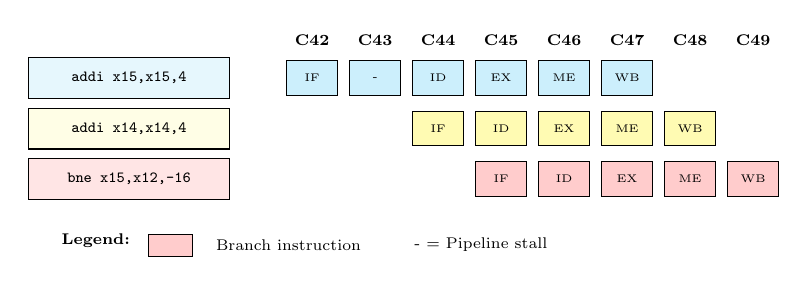
\begin{tikzpicture}[
        scale=0.80,
        transform shape,
        instruction/.style={rectangle, draw, minimum width=3.2cm, minimum height=0.65cm, font=\ttfamily\scriptsize},
        cycle/.style={font=\scriptsize\bfseries}
    ]
    % Cycle numbers
    \foreach \i in {42,...,49} {
        \node[cycle] at (0.3 + 1.0*\i - 41.0, 1.6) {C\i};
    }

    % Instruction labels
    \node[instruction, anchor=east, fill=cyan!10] at (0, 1.0) {addi x15,x15,4};
    \node[instruction, anchor=east, fill=yellow!10] at (0, 0.2) {addi x14,x14,4};
    \node[instruction, anchor=east, fill=red!10] at (0, -0.6) {bne x15,x12,-16};

    % Timelines (matches the cycle discussion in text)
    % addi x15,x15,4 (includes one bubble as in the screenshot)
    \foreach \i/\stage in {42/IF, 43/-, 44/ID, 45/EX, 46/ME, 47/WB} {
        \node[draw, fill=cyan!20, minimum width=0.8cm, minimum height=0.55cm] at (0.3 + 1.0*\i - 41.0, 1.0) {\tiny\stage};
    }

    % addi x14,x14,4
    \foreach \i/\stage in {44/IF, 45/ID, 46/EX, 47/ME, 48/WB} {
        \node[draw, fill=yellow!30, minimum width=0.8cm, minimum height=0.55cm] at (0.3 + 1.0*\i - 41.0, 0.2) {\tiny\stage};
    }

    % bne x15,x12,-16
    \foreach \i/\stage in {45/IF, 46/ID, 47/EX, 48/ME, 49/WB} {
        \node[draw, fill=red!20, minimum width=0.8cm, minimum height=0.55cm] at (0.3 + 1.0*\i - 41.0, -0.6) {\tiny\stage};
    }

    % Legend (same look/placement style as later figures)
    \node[font=\scriptsize\bfseries, anchor=north west] at (-2.8, -1.35) {\textbf{Legend:}};
    \node[draw, fill=red!20, minimum width=0.7cm, minimum height=0.35cm, anchor=west] at (-1.3, -1.65) {};
    \node[font=\scriptsize, anchor=west] at (-0.35, -1.65) {Branch instruction};
    \node[font=\scriptsize, anchor=west] at (2.8, -1.65) {- = Pipeline stall};
    \end{tikzpicture}
    \caption{Forwarding into \textbf{EX}: \texttt{bne x15, x12, -16} uses the updated \texttt{x15} before \texttt{addi x15, x15, 4} reaches \textbf{WB}.}
    \label{fig:forwarding_alu_branch}
\end{figure}

\subsubsection{Load\textendash use hazard (stall)}
Not all RAW hazards are eliminated. The classic special case is when an instruction loads a value from memory and the very next instruction immediately needs it. In the loop body, \texttt{lw x13, 0(x15)} loads an array element into \texttt{x13} and the next instruction \texttt{sw x13, 0(x14)} stores that same value to another address. In the pipeline diagram, \texttt{lw x13, 0(x15)} proceeds normally with \textbf{MEM} at cycle 43 and \textbf{WB} at cycle 44. The following store shows an explicit one\textendash cycle bubble (\texttt{-}) at cycle 43, i.e., it goes \textbf{IF} 41 $\rightarrow$ \textbf{ID} 42 $\rightarrow$ \texttt{-} 43 $\rightarrow$ \textbf{EX} 44 $\rightarrow$ \textbf{MEM} 45 $\rightarrow$ \textbf{WB} 46. This stall occurs because the loaded data is only available after the load's memory access (end of \textbf{MEM}), so the pipeline must delay the consumer so that the correct data can be forwarded in time. Therefore, the processor supports forwarding, but still pays a one\textendash cycle penalty for back\textendash to\textendash back load\textendash use patterns.

\begin{figure}[H]
    \centering
    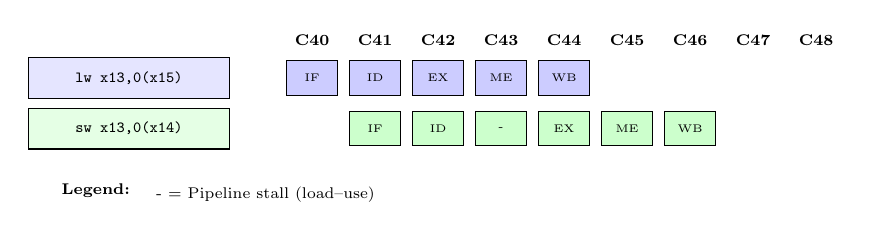
\begin{tikzpicture}[
        scale=0.80,
        transform shape,
        instruction/.style={rectangle, draw, minimum width=3.2cm, minimum height=0.65cm, font=\ttfamily\scriptsize},
        cycle/.style={font=\scriptsize\bfseries}
    ]
    \foreach \i in {40,...,48} {
        \node[cycle] at (0.3 + 1.0*\i - 39.0, 1.6) {C\i};
    }

    \node[instruction, anchor=east, fill=blue!10] at (0, 1.0) {lw x13,0(x15)};
    \node[instruction, anchor=east, fill=green!10] at (0, 0.2) {sw x13,0(x14)};

    \foreach \i/\stage in {40/IF, 41/ID, 42/EX, 43/ME, 44/WB} {
        \node[draw, fill=blue!20, minimum width=0.8cm, minimum height=0.55cm] at (0.3 + 1.0*\i - 39.0, 1.0) {\tiny\stage};
    }
    \foreach \i/\stage in {41/IF, 42/ID, 43/-, 44/EX, 45/ME, 46/WB} {
        \node[draw, fill=green!20, minimum width=0.8cm, minimum height=0.55cm] at (0.3 + 1.0*\i - 39.0, 0.2) {\tiny\stage};
    }

    \node[font=\scriptsize\bfseries, anchor=north west] at (-2.8, -0.55) {\textbf{Legend:}};
    \node[font=\scriptsize, anchor=west] at (-1.3, -0.85) {- = Pipeline stall (load\textendash use)};
    \end{tikzpicture}
    \caption{Load\textendash use hazard: one\textendash cycle bubble between \texttt{lw x13, 0(x15)} and \texttt{sw x13, 0(x14)}.}
    \label{fig:load_use_stall}
\end{figure}

\subsubsection{Control hazard}
The loop branch \texttt{bne x15, x12, -16} introduces a control hazard. In a simple 5\textendash stage design, the branch decision is typically resolved in \textbf{EX}, so some instructions fetched in the meantime may belong to the wrong path. In our pipeline diagram (in Figure~\ref{fig:control_hazard}), immediately after the branch enters the pipeline (\textbf{IF} at cycle 45), subsequent instructions such as \texttt{addi x9, x0, 0} appear only in early stages (\textbf{IF} at cycle 46, \textbf{ID} at cycle 47) and then disappear (they do not progress to \textbf{EX/MEM/WB}) within the shown window. This is consistent with the instruction being fetched/decoded but later flushed when the taken branch redirects the PC. This behavior matches a basic pipeline with no dynamic branch prediction and branch resolution late enough to waste at least some fetch/decode work per taken loop branch.

\begin{figure}[H]
    \centering
    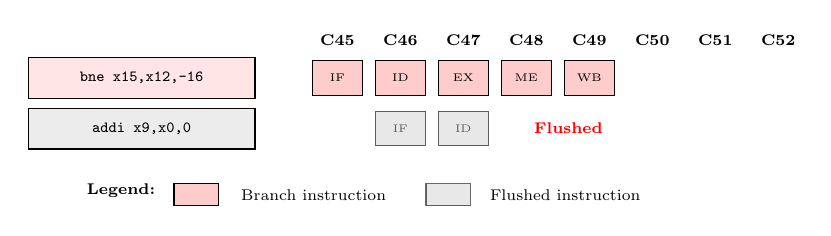
\begin{tikzpicture}[
        scale=0.80,
        transform shape,
        instruction/.style={rectangle, draw, minimum width=3.6cm, minimum height=0.65cm, font=\ttfamily\scriptsize},
        cycle/.style={font=\scriptsize\bfseries}
    ]
    \foreach \i in {45,...,52} {
        \node[cycle] at (0.3 + 1.0*\i - 44.0, 1.6) {C\i};
    }

    \node[instruction, anchor=east, fill=red!10] at (0, 1.0) {bne x15,x12,-16};
    \node[instruction, anchor=east, fill=gray!15] at (0, 0.2) {addi x9,x0,0};

    \foreach \i/\stage in {45/IF, 46/ID, 47/EX, 48/ME, 49/WB} {
        \node[draw, fill=red!20, minimum width=0.8cm, minimum height=0.55cm] at (0.3 + 1.0*\i - 44.0, 1.0) {\tiny\stage};
    }

    % Fall-through instruction appears only in early stages and is flushed
    \foreach \i/\stage in {46/IF, 47/ID} {
        \node[draw, fill=gray!30, minimum width=0.8cm, minimum height=0.55cm, opacity=0.6] at (0.3 + 1.0*\i - 44.0, 0.2) {\tiny\stage};
    }
    \node[font=\scriptsize\color{red}, anchor=west] at (0.3 + 1.0*48 - 44.0, 0.2) {\textbf{Flushed}};

    \node[font=\scriptsize\bfseries, anchor=north west] at (-2.8, -0.55) {\textbf{Legend:}};
    \node[draw, fill=red!20, minimum width=0.7cm, minimum height=0.35cm, anchor=west] at (-1.3, -0.85) {};
    \node[font=\scriptsize, anchor=west] at (-0.35, -0.85) {Branch instruction};
    \node[draw, fill=gray!30, minimum width=0.7cm, minimum height=0.35cm, opacity=0.6, anchor=west] at (2.7, -0.85) {};
    \node[font=\scriptsize, anchor=west] at (3.6, -0.85) {Flushed instruction};
    \end{tikzpicture}
    \caption{Taken\textendash branch control hazard: fall\textendash through instruction is fetched but flushed after \texttt{bne x15, x12, -16} redirects the PC.}
    \label{fig:control_hazard}
\end{figure}

\subsubsection{Structural hazard}
The processor does not need to handle structural hazards since it has enough resources to execute all
instructions without contention. For example, there are separate instruction and data memory, so there
are no structural hazards between instruction fetch and memory access stages. Also, there are enough
functional units to handle all arithmetic and logic operations without contention.

\subsubsection{Capabilities summary}
The 5\textendash stage CPU executes one instruction per cycle in the ideal case, but uses hazard logic to maintain correctness. The pipeline supports data forwarding into \textbf{EX}, allowing back\textendash to\textendash back ALU/branch/address computations to proceed without waiting for \textbf{WB} (demonstrated by \texttt{addi x15, x15, 4} feeding \texttt{bne x15, x12, -16} one cycle later in Figure~\ref{fig:forwarding_alu_branch}). However, the pipeline still has to pause in the classic load\textendash use case: when a value is loaded with \texttt{lw} and the very next instruction needs that value, it cannot always proceed immediately because the data is only ready after the load's \textbf{MEM} stage. This shows up as a stall in Figure~\ref{fig:load_use_stall}. Branches introduce a similar inefficiency on the control side: because the branch outcome is only known once the branch is resolved, the processor may fetch and decode one or more instructions along the wrong path and then discard them, as illustrated in Figure~\ref{fig:control_hazard}.

\subsection{How the simulator detects completion}
The simulator determines program completion by observing a terminating environment call. In the executed instruction stream, the program eventually reaches the \texttt{\_start} termination sequence where the register \texttt{a7} (\texttt{x17}) is set to a specific value and then an \texttt{ecall} instruction is executed. In Ripes \cite{ripes_repo}, \texttt{ecall} implements a set of simulator\textendash defined ``environment calls''; when \texttt{a7 = 10}, the call corresponds to \emph{exit}, so Ripes halts simulation and reports program completion.

In the RISC\textendash V ISA, \texttt{ecall} (environment call) is an instruction used to request a service from the execution environment, typically the operating system or a runtime monitor, by raising an environment\textendash call exception to a higher\textendash privileged handler \cite{riscv_unpriv_isa}. Which service is requested (e.g., exit, print, read) is not fixed by the ISA itself; it is defined by the ABI/runtime convention, typically using designated registers to pass a syscall number and arguments \cite{borza_ecalls_syscalls}. In Ripes, this mechanism is reused to provide basic I/O and termination services inside the simulator, with the call selector stored in \texttt{a7}.

\subsubsection{Pipeline\textendash level view}
From the pipeline diagram, program completion is visible because the terminating sequence \texttt{addi x17, x0, 10} followed by \texttt{ecall} appears in the executed instruction stream. In the early trace window (Figure~\ref{fig:ecall_early}), the simulator has fetched the instructions that prepare the exit call (setting \texttt{a7/x17} to 10) and then fetches the \texttt{ecall}. In the final trace window at the end of execution (Figure~\ref{fig:ecall_end}), \texttt{ecall} progresses through the pipeline and the simulation stops afterwards because the program has explicitly requested termination.

The \texttt{ecall} row may show extra delay cycles (\texttt{-}) before completing (Figure~\ref{fig:ecall_end}). This reflects how Ripes processes an environment call: after recognizing an exit request, it stops fetching new instructions, lets the pipeline drain and then marks the simulation as finished. For that reason, completion is not inferred from ``falling off'' the end of memory or returning from \texttt{main}; it is triggered by the explicit exit environment call.

\begin{figure}[H]
    \centering
    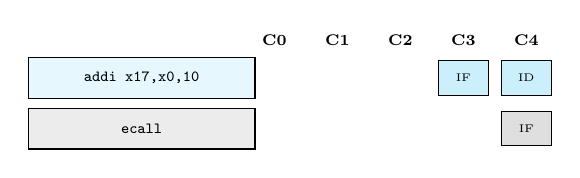
\begin{tikzpicture}[
        scale=0.80,
        transform shape,
        instruction/.style={rectangle, draw, minimum width=3.6cm, minimum height=0.65cm, font=\ttfamily\scriptsize},
        cycle/.style={font=\scriptsize\bfseries}
    ]
    \foreach \i in {0,...,4} {
        \node[cycle] at (0.3 + 1.0*\i, 1.6) {C\i};
    }

    \node[instruction, anchor=east, fill=cyan!10] at (0, 1.0) {addi x17,x0,10};
    \node[instruction, anchor=east, fill=gray!15] at (0, 0.2) {ecall};

    % Early trace window (as in screenshot): addi visible at IF then ID; ecall just fetched
    \foreach \i/\stage in {3/IF, 4/ID} {
        \node[draw, fill=cyan!20, minimum width=0.8cm, minimum height=0.55cm] at (0.3 + 1.0*\i, 1.0) {\tiny\stage};
    }
    \foreach \i/\stage in {4/IF} {
        \node[draw, fill=gray!25, minimum width=0.8cm, minimum height=0.55cm] at (0.3 + 1.0*\i, 0.2) {\tiny\stage};
    }
    \end{tikzpicture}
    \caption{Early exit sequence in the trace: \texttt{addi x17, x0, 10} then \texttt{ecall}.}
    \label{fig:ecall_early}
\end{figure}

\begin{figure}[H]
    \centering
    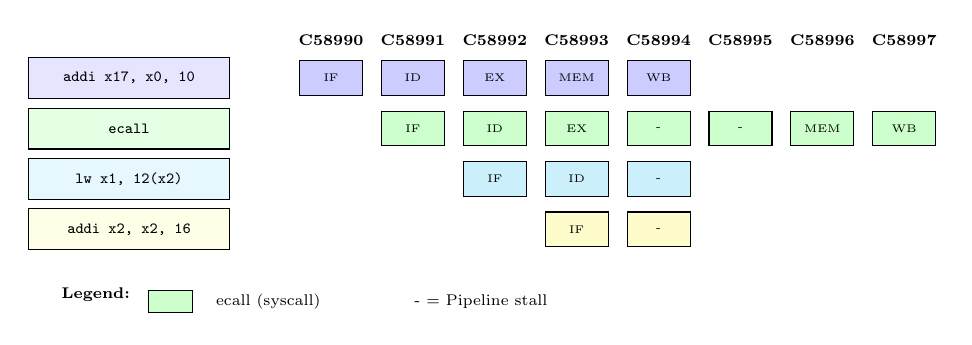
\begin{tikzpicture}[
        scale=0.80,
        transform shape,
        instruction/.style={rectangle, draw, minimum width=3.2cm, minimum height=0.65cm, font=\ttfamily\scriptsize},
        cycle/.style={font=\scriptsize\bfseries}
    ]

    % Cycle numbers: C58990 through C58998 (9 cycles)
    \foreach \i [count=\ci from 1] in {58990,58991,58992,58993,58994,58995,58996,58997} {
        \node[cycle] at (0.3 + 1.3*\ci, 1.6) {C\i};
    }

    % Instruction labels (anchor=east, left of diagram)
    \node[instruction, anchor=east, fill=blue!10]   at (0, 1.0)  {addi x17, x0, 10};
    \node[instruction, anchor=east, fill=green!10] at (0, 0.2)  {ecall};
    \node[instruction, anchor=east, fill=cyan!10]    at (0, -0.6) {lw x1, 12(x2)};
    \node[instruction, anchor=east, fill=yellow!10]  at (0, -1.4) {addi x2, x2, 16};

    % --------------------------------------------------
    % addi x17, x0, 10
    % C58990=IF(1), C58991=ID(2), C58992=EX(3), C58993=MEM(4), C58994=WB(5)
    \foreach \ci/\stage in {1/IF, 2/ID, 3/EX, 4/MEM, 5/WB} {
        \node[draw, fill=blue!20, minimum width=1cm, minimum height=0.55cm]
            at (0.3 + 1.3*\ci, 1.0) {\tiny\stage};
    }

    % --------------------------------------------------
    % ecall
    % C58991=IF(2), C58992=ID(3), C58993=EX(4), C58994=-(5), C58995=-(6), C58996=MEM(7), C58997=WB(8)
    \foreach \ci/\stage in {2/IF, 3/ID, 4/EX, 5/{-}, 6/{-}, 7/MEM, 8/WB} {
        \node[draw, fill=green!20, minimum width=1cm, minimum height=0.55cm]
            at (0.3 + 1.3*\ci, 0.2) {\tiny\stage};
    }

    % --------------------------------------------------
    % lw x1, 12(x2)
    % C58992=IF(3), C58993=ID(4), C58994=-(5)
    \foreach \ci/\stage in {3/IF, 4/ID, 5/{-}} {
        \node[draw, fill=cyan!20, minimum width=1cm, minimum height=0.55cm]
            at (0.3 + 1.3*\ci, -0.6) {\tiny\stage};
    }

    % --------------------------------------------------
    % addi x2, x2, 16
    % C58993=IF(4), C58994=-(5)
    \foreach \ci/\stage in {4/IF, 5/{-}} {
        \node[draw, fill=yellow!20, minimum width=1cm, minimum height=0.55cm]
            at (0.3 + 1.3*\ci, -1.4) {\tiny\stage};
    }

    % Legend
    \node[font=\scriptsize\bfseries, anchor=north west] at (-2.8, -2.2) {\textbf{Legend:}};
    \node[draw, fill=green!20, minimum width=0.7cm, minimum height=0.35cm, anchor=west] at (-1.3, -2.55) {};
    \node[font=\scriptsize, anchor=west] at (-0.35, -2.55) {ecall (syscall)};
    \node[font=\scriptsize, anchor=west] at (2.8, -2.55) {- = Pipeline stall};

    \end{tikzpicture}
    \caption{End of execution: final \texttt{addi x17, x0, 10} and \texttt{ecall} in the trace (simulation halts after \texttt{ecall}).}
    \label{fig:ecall_pipeline}
\end{figure}

\section{Branches and Multiple-Issue}

This section examines the performance of two pipelined processor
configurations—a 5-stage single-issue and a 6-stage dual-issue
processor—by simulating the execution of an insertion sort ELF binary.
The analysis focuses on pipeline stalls, branch handling, data hazards,
and overall CPI efficiency. Through systematic observation
of pipeline diagrams and simulation results,
we identify key performance bottlenecks and discuss how architectural choices
influence execution behavior.
\subsection{5-Stage Pipeline Analysis}

Before examining the specific execution details of the insertion sort program, it is essential to understand the foundational architecture of the processor under analysis. The simulated processor implements the classic 5-stage RISC pipeline design, as visually depicted in the architectural diagram provided by the \textbf{Ripes} simulator in Figure~\ref{fig:5stage_pipeline}. This canonical design serves as the baseline for our performance evaluation.

\begin{figure}[h]
    \centering
    \includegraphics[width=0.9\linewidth]{img/5-stage_RISC-V_processor.jpeg}
    \caption{Diagram of the 5-stage RISC-V pipeline architecture }
    \label{fig:5stage_pipeline}
\end{figure}

The pipeline consists of the following stages:
\begin{enumerate}
    \item \textbf{Instruction Fetch (IF):} Retrieve the next instruction from memory.
    \item \textbf{Instruction Decode (ID):} Decode the instruction and read register values.
    \item \textbf{Execute (EX):} Perform arithmetic/logic operations or calculate addresses.
    \item \textbf{Memory Access (ME):} Access data memory for load/store operations.
    \item \textbf{Write Back (WB):} Write results back to the register file.
\end{enumerate}

This design aims to achieve a throughput of one instruction per cycle (CPI = 1.0). However,
hazards disrupt this flow, causing stalls and flushes that degrade performance, as observed
in the following analysis.
\subsubsection{Incomplete Instructions in the Pipeline}

When examining the pipeline diagram of the insertion sort execution, several instructions fail to complete their execution. Figure~\ref{fig:branch_flushing} illustrates a representative example where two \texttt{addi} instructions are flushed from the pipeline.

\begin{figure}[htbp]
\centering
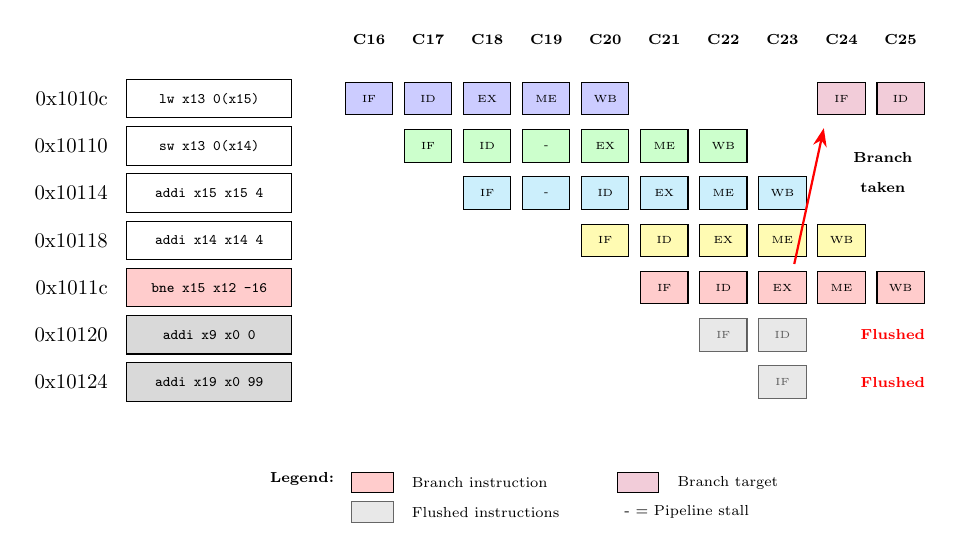
\begin{tikzpicture}[
    scale=0.75,
    transform shape,
    instruction/.style={rectangle, draw, minimum width=2.8cm, minimum height=0.65cm, font=\ttfamily\scriptsize},
    stage/.style={font=\scriptsize\bfseries},
    cycle/.style={font=\scriptsize\bfseries},
    arrow/.style={->, >=Stealth, thick, red}
]

% Cycle numbers at top
\foreach \i in {16,...,25} {
    \node[cycle] at (0.3 + 1.0*\i -15.0, 5.0) {C\i};
}

\node[ anchor=east] at (-3, 4.0) {0x1010c};
\node[ anchor=east] at (-3, 3.2) {0x10110};
\node[ anchor=east] at (-3, 2.4) {0x10114};
\node[ anchor=east] at (-3, 1.6) {0x10118};
\node[ anchor=east] at (-3, 0.8) {0x1011c};
\node[ anchor=east] at (-3, 0.0) {0x10120};
\node[ anchor=east] at (-3, -0.8) {0x10124};
% Instructions labels on the left

\node[instruction, anchor=east] at (0, 4.0) {lw x13 0(x15)};
\node[instruction, anchor=east] at (0, 3.2) {sw x13 0(x14)};
\node[instruction, anchor=east] at (0, 2.4) {addi x15 x15 4};
\node[instruction, anchor=east] at (0, 1.6) {addi x14 x14 4};
\node[instruction, anchor=east, fill=red!20] at (0, 0.8) {bne x15 x12 -16};
\node[instruction, anchor=east, fill=gray!30] at (0, 0.0) {addi x9 x0 0};
\node[instruction, anchor=east, fill=gray!30] at (0, -0.8) {addi x19 x0 99};

% lw x13 0 x15
\foreach \i/\stage in {1/IF, 2/ID, 3/EX, 4/ME, 5/WB, 9/IF, 10/ID} {
    \ifnum \i > 5
        \node[draw, fill=purple!20, minimum width=0.8cm, minimum height=0.55cm] at (0.3 + 1.0*\i, 4.0) {\tiny\stage};
    \else
        \node[draw, fill=blue!20, minimum width=0.8cm, minimum height=0.55cm] at (0.3 + 1.0*\i, 4.0) {\tiny\stage};
    \fi
}

% sw x13 0 x14
\foreach \i/\stage in {2/IF, 3/ID, 4/-, 5/EX, 6/ME, 7/WB} {
    \node[draw, fill=green!20, minimum width=0.8cm, minimum height=0.55cm] at (0.3 + 1.0*\i, 3.2) {\tiny\stage};
}

% addi x15 x15 4
\foreach \i/\stage in {3/IF, 4/-, 5/ID, 6/EX, 7/ME, 8/WB} {
    \node[draw, fill=cyan!20, minimum width=0.8cm, minimum height=0.55cm] at (0.3 + 1.0*\i, 2.4) {\tiny\stage};
}

% addi x14 x14 4 (shifted one cycle to the right)
\foreach \i/\stage in {5/IF, 6/ID, 7/EX, 8/ME, 9/WB} {
    \node[draw, fill=yellow!30, minimum width=0.8cm, minimum height=0.55cm] at (0.3 + 1.0*\i, 1.6) {\tiny\stage};
}

% bne x15 x12 -16 (branch taken) - shifted one cycle
\foreach \i/\stage in {6/IF, 7/ID, 8/EX, 9/ME, 10/WB} {
    \node[draw, fill=red!20, minimum width=0.8cm, minimum height=0.55cm] at (0.3 + 1.0*\i, 0.8) {\tiny\stage};
}

% addi x9 x0 0 (FLUSHED) - shifted one cycle
\foreach \i/\stage in {7/IF, 8/ID} {
    \node[draw, fill=gray!30, minimum width=0.8cm, minimum height=0.55cm, opacity=0.6] at (0.3 + 1.0*\i, 0.0) {\tiny\stage};
}
\node[font=\scriptsize\color{red}, anchor=west] at (9.5, 0.0) {\textbf{Flushed}};

% addi x19 x0 99 (FLUSHED) - shifted one cycle
\foreach \i/\stage in {8/IF} {
    \node[draw, fill=gray!30, minimum width=0.8cm, minimum height=0.55cm, opacity=0.6] at (0.3 + 1.0*\i, -0.8) {\tiny\stage};
}
\node[font=\scriptsize\color{red}, anchor=west] at (9.5, -0.8) {\textbf{Flushed}};


% Update the purple branch target stages


% Arrow showing branch resolution - adjusted position
\draw[arrow] (8.5, 1.2) -- (9, 3.5);
\node[font=\scriptsize] at (10, 3.0) {\textbf{Branch}};
\node[font=\scriptsize] at (10, 2.5) {\textbf{taken}};

% Legend
\node[font=\scriptsize\bfseries, anchor=north west] at (-0.5, -2.2) {\textbf{Legend:}};

\node[draw, fill=red!20, minimum width=0.7cm, minimum height=0.35cm, anchor=west] at (1.0, -2.5) {};
\node[font=\scriptsize, anchor=west] at (1.9, -2.5) {Branch instruction};

\node[draw, fill=gray!30, minimum width=0.7cm, minimum height=0.35cm, opacity=0.6, anchor=west] at (1.0, -3.0) {};
\node[font=\scriptsize, anchor=west] at (1.9, -3.0) {Flushed instructions};

\node[draw, fill=purple!20, minimum width=0.7cm, minimum height=0.35cm, anchor=west] at (5.5, -2.5) {};
\node[font=\scriptsize, anchor=west] at (6.4, -2.5) {Branch target};

\node[font=\scriptsize, anchor=west] at (5.5, -3.0) {- = Pipeline stall};

\end{tikzpicture}
\caption{Pipeline behavior showing instruction flushing when branch is taken.}
\label{fig:branch_flushing}
\end{figure}

The incomplete instructions occur due to \textbf{control hazards} caused by branch instructions. When a branch is taken, instructions that were speculatively fetched from the sequential path (fall-through) must be discarded. In the example shown, the two \texttt{addi} instructions (\texttt{addi x9 x0 0} and \texttt{addi x19 x0 99}) enter the pipeline after the branch instruction but before the branch outcome is determined. Once the branch is resolved as taken (in the EX stage), these instructions are flushed from the pipeline as they represent incorrect speculative execution. The processor must then begin fetching from the correct branch target address, which in this case returns to the \texttt{lw x13 0 x15} instruction, indicating a loop structure.

This flushing mechanism is necessary to maintain correct program semantics: executing instructions from the wrong path would produce incorrect results. The cost of this mechanism is the branch penalty—cycles wasted on instructions that do not contribute to program progress.

Additionally, the pipeline diagram reveals \textbf{pipeline stalls} (indicated by dashes "-" in the diagram), which occur due to \textbf{Data hazards} (data dependencies). For instance, the \texttt{sw x13 0 x14} instruction stalls in the ID stage because it depends on the result of the previous \texttt{lw} instruction, which hasn't yet completed its ME stage where the data is loaded.


\subsubsection{Branch Prediction Mechanism}
Based on the observed pipeline behavior of the first loop in \texttt{< main >} (Figure \ref{fig:branch_flushing_extended} ), the processor does \textbf{not appear to have a sophisticated branch predictor}.
The consistent patterns observed across all branch instructions indicates the absence of a dynamic branch predictor in this processor design. This conclusion is supported by several key observations:
\begin{itemize}
    \item \textbf{Flushing Pattern}: Every taken branch exhibits identical flushing behavior, regardless of execution history. This suggests a static approach rather than adaptive learning.

    \item \textbf{No Learning Observed}: In a typical dynamic branch predictor (such as a two-bit saturating counter or branch history table), we would expect:
    \begin{enumerate}
        \item \textbf{Initial iterations}: Flushes would occur as the predictor learns branch behavior
        \item \textbf{Subsequent iterations}: After 2 executions, the predictor would accurately predict the branch direction, eliminating flushes
    \end{enumerate}
    The insertion sort algorithm contains loop branches that are typically taken many times consecutively. A competent dynamic predictor would quickly learn this pattern and avoid flushing after the initial learning phase.

    \item \textbf{Statistical Evidence}: Analysis of the pipeline trace reveals that branches exhibit the same 2-cycle penalty (flushing 2 instructions) throughout execution, with no improvement over time. This static penalty pattern is characteristic of processors without branch prediction or with always-not-taken static prediction.
\end{itemize}

To illustrate what we would expect with a dynamic branch predictor, consider the following theoretical behavior pattern for a loop branch:

\begin{table}[H]
\centering
\vspace{0.3cm}
\renewcommand{\arraystretch}{1.4}
\scalebox{0.85}{ % Scale the entire table to 85% of original size
\begin{tabular}{|c|c|c|c|c|}
\hline
\rowcolor{blue!20}
\textbf{Branch Iteration} &
\textbf{Predicted Outcome} &
\textbf{Actual Outcome} &
\textbf{Pipeline Flush} &
\textbf{Predictor State Update} \\
\hline
\rowcolor{red!30}
1st & Strongly Not Taken (initial) & Taken & Yes (2 instructions) & Learn → Weakly Not Taken\\
\hline
\rowcolor{red!10}
2nd & Weakly Not Taken  & Taken & Yes (2 instructions) & Learn → Weakly Taken \\
\hline
\rowcolor{green!10}
3rd & Weakly Taken & Taken & No (correct prediction) & Learn → Strongly Taken \\
\hline
\rowcolor{green!30}
4th & Strongly Taken & Taken & No (correct prediction) & Maintain Strongly Taken \\
\hline
\rowcolor{green!30}
5th+ & Strongly Taken & Taken & No (correct prediction) & Maintain Strongly Taken \\
\hline
\end{tabular}
} % End of scalebox
\caption{Expected behavior of a two-bit saturating counter branch predictor}
\label{tab:branch_predictor_behavior}
\end{table}

Since our observations show \textbf{consistent flushing across all iterations}, we can conclude that no such learning mechanism exists in this implementation.
\begin{figure}[htbp]
\centering
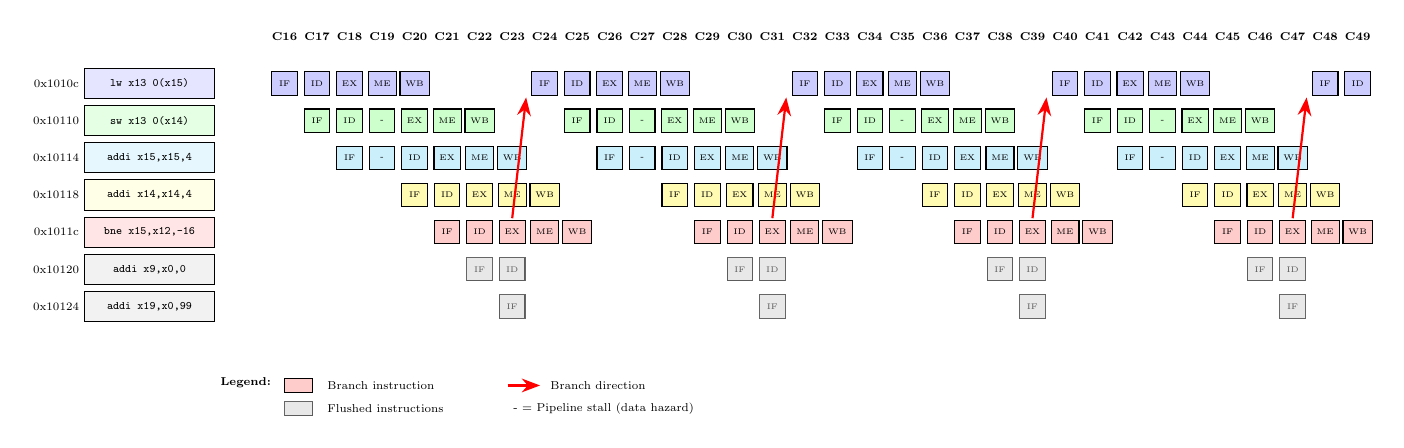
\begin{tikzpicture}[
    scale=0.59,
    transform shape,
    instruction/.style={rectangle, draw, minimum width=2.8cm, minimum height=0.65cm, font=\ttfamily\scriptsize},
    stage/.style={font=\scriptsize\bfseries},
    cycle/.style={font=\scriptsize\bfseries},
    arrow/.style={->, >= Stealth, thick, red}
]

% Cycle numbers at top - extended to show multiple iterations
\foreach \i in {16,...,49} {
    \node[cycle] at (4.8 + 0.7*\i-15, 5.0) {C\i};
}

% Program counter addresses
\node[anchor=east, font=\scriptsize] at (-3.3, 4.0) {0x1010c};
\node[anchor=east, font=\scriptsize] at (-3.3, 3.2) {0x10110};
\node[anchor=east, font=\scriptsize] at (-3.3, 2.4) {0x10114};
\node[anchor=east, font=\scriptsize] at (-3.3, 1.6) {0x10118};
\node[anchor=east, font=\scriptsize] at (-3.3, 0.8) {0x1011c};
\node[anchor=east, font=\scriptsize] at (-3.3, 0.0) {0x10120};
\node[anchor=east, font=\scriptsize] at (-3.3, -0.8) {0x10124};

% Instructions labels on the left
\node[instruction, anchor=east,fill=blue!10] at (-0.5, 4.0) {lw x13 0(x15)};
\node[instruction, anchor=east,fill=green!10] at (-0.5, 3.2) {sw x13 0(x14)};
\node[instruction, anchor=east,fill=cyan!10] at (-0.5, 2.4) {addi x15,x15,4};
\node[instruction, anchor=east,fill=yellow!10] at (-0.5, 1.6) {addi x14,x14,4};
\node[instruction, anchor=east, fill=red!10] at (-0.5, 0.8) {bne x15,x12,-16};
\node[instruction, anchor=east, fill=gray!10] at (-0.5, 0.0) {addi x9,x0,0};
\node[instruction, anchor=east, fill=gray!10] at (-0.5, -0.8) {addi x19,x0,99};

% First iteration: lw x13 0(x15)
\foreach \i/\stage in {1/IF, 2/ID, 3/EX, 4/ME, 5/WB} {
    \node[draw, fill=blue!20, minimum width=0.55cm, minimum height=0.5cm] at (0.3 + 0.7*\i, 4.0) {\tiny\stage};
}

% First iteration: sw x13 0(x14)
\foreach \i/\stage in {2/IF, 3/ID, 4/-, 5/EX, 6/ME, 7/WB} {
    \node[draw, fill=green!20, minimum width=0.55cm, minimum height=0.5cm] at (0.3 + 0.7*\i, 3.2) {\tiny\stage};
}

% First iteration: addi x15 x15 4
\foreach \i/\stage in {3/IF, 4/-, 5/ID, 6/EX, 7/ME, 8/WB} {
    \node[draw, fill=cyan!20, minimum width=0.55cm, minimum height=0.5cm] at (0.3 + 0.7*\i, 2.4) {\tiny\stage};
}

% First iteration: addi x14 x14 4
\foreach \i/\stage in {5/IF, 6/ID, 7/EX, 8/ME, 9/WB} {
    \node[draw, fill=yellow!30, minimum width=0.55cm, minimum height=0.5cm] at (0.3 + 0.7*\i, 1.6) {\tiny\stage};
}

% First iteration: bne (branch taken)
\foreach \i/\stage in {6/IF, 7/ID, 8/EX, 9/ME, 10/WB} {
    \node[draw, fill=red!20, minimum width=0.55cm, minimum height=0.5cm] at (0.3 + 0.7*\i, 0.8) {\tiny\stage};
}

% First iteration: addi x9 (FLUSHED)
\foreach \i/\stage in {7/IF, 8/ID} {
    \node[draw, fill=gray!30, minimum width=0.55cm, minimum height=0.5cm, opacity=0.6] at (0.3 + 0.7*\i, 0.0) {\tiny\stage};
}

% First iteration: addi x19 (FLUSHED)
\foreach \i/\stage in {8/IF} {
    \node[draw, fill=gray!30, minimum width=0.55cm, minimum height=0.5cm, opacity=0.6] at (0.3 + 0.7*\i, -0.8) {\tiny\stage};
}

% Second iteration: lw x13 0(x15)
\foreach \i/\stage in {9/IF, 10/ID, 11/EX, 12/ME, 13/WB} {
    \node[draw, fill=blue!20, minimum width=0.55cm, minimum height=0.5cm] at (0.3 + 0.7*\i, 4.0) {\tiny\stage};
}

% Second iteration: sw x13 0(x14)
\foreach \i/\stage in {10/IF, 11/ID, 12/-, 13/EX, 14/ME, 15/WB} {
    \node[draw, fill=green!20, minimum width=0.55cm, minimum height=0.5cm] at (0.3 + 0.7*\i, 3.2) {\tiny\stage};
}

% Second iteration: addi x15 x15 4
\foreach \i/\stage in {11/IF, 12/-, 13/ID, 14/EX, 15/ME, 16/WB} {
    \node[draw, fill=cyan!20, minimum width=0.55cm, minimum height=0.5cm] at (0.3 + 0.7*\i, 2.4) {\tiny\stage};
}

% Second iteration: addi x14 x14 4
\foreach \i/\stage in {13/IF, 14/ID, 15/EX, 16/ME, 17/WB} {
    \node[draw, fill=yellow!30, minimum width=0.55cm, minimum height=0.5cm] at (0.3 + 0.7*\i, 1.6) {\tiny\stage};
}

% Second iteration: bne (branch taken)
\foreach \i/\stage in {14/IF, 15/ID, 16/EX, 17/ME, 18/WB} {
    \node[draw, fill=red!20, minimum width=0.55cm, minimum height=0.5cm] at (0.3 + 0.7*\i, 0.8) {\tiny\stage};
}

% Second iteration: addi x9 (FLUSHED)
\foreach \i/\stage in {15/IF, 16/ID} {
    \node[draw, fill=gray!30, minimum width=0.55cm, minimum height=0.5cm, opacity=0.6] at (0.3 + 0.7*\i, 0.0) {\tiny\stage};
}

% Second iteration: addi x19 (FLUSHED)
\foreach \i/\stage in {16/IF} {
    \node[draw, fill=gray!30, minimum width=0.55cm, minimum height=0.5cm, opacity=0.6] at (0.3 + 0.7*\i, -0.8) {\tiny\stage};
}

% Third iteration: lw x13 0(x15)
\foreach \i/\stage in {17/IF, 18/ID, 19/EX, 20/ME, 21/WB} {
    \node[draw, fill=blue!20, minimum width=0.55cm, minimum height=0.5cm] at (0.3 + 0.7*\i, 4.0) {\tiny\stage};
}

% Third iteration: sw x13 0(x14)
\foreach \i/\stage in {18/IF, 19/ID, 20/-, 21/EX, 22/ME, 23/WB} {
    \node[draw, fill=green!20, minimum width=0.55cm, minimum height=0.5cm] at (0.3 + 0.7*\i, 3.2) {\tiny\stage};
}

% Third iteration: addi x15 x15 4
\foreach \i/\stage in {19/IF, 20/-, 21/ID, 22/EX, 23/ME, 24/WB} {
    \node[draw, fill=cyan!20, minimum width=0.55cm, minimum height=0.5cm] at (0.3 + 0.7*\i, 2.4) {\tiny\stage};
}

% Third iteration: addi x14 x14 4
\foreach \i/\stage in {21/IF, 22/ID, 23/EX, 24/ME, 25/WB} {
    \node[draw, fill=yellow!30, minimum width=0.55cm, minimum height=0.5cm] at (0.3 + 0.7*\i, 1.6) {\tiny\stage};
}

% Third iteration: bne (branch taken)
\foreach \i/\stage in {22/IF, 23/ID, 24/EX, 25/ME, 26/WB} {
    \node[draw, fill=red!20, minimum width=0.55cm, minimum height=0.5cm] at (0.3 + 0.7*\i, 0.8) {\tiny\stage};
}

% Third iteration: addi x9 (FLUSHED)
\foreach \i/\stage in {23/IF, 24/ID} {
    \node[draw, fill=gray!30, minimum width=0.55cm, minimum height=0.5cm, opacity=0.6] at (0.3 + 0.7*\i, 0.0) {\tiny\stage};
}

% Third iteration: addi x19 (FLUSHED)
\foreach \i/\stage in {24/IF} {
    \node[draw, fill=gray!30, minimum width=0.55cm, minimum height=0.5cm, opacity=0.6] at (0.3 + 0.7*\i, -0.8) {\tiny\stage};
}

% Fourth iteration: lw x13 0(x15)
\foreach \i/\stage in {25/IF, 26/ID, 27/EX, 28/ME, 29/WB} {
    \node[draw, fill=blue!20, minimum width=0.55cm, minimum height=0.5cm] at (0.3 + 0.7*\i, 4.0) {\tiny\stage};
}

% Fourth iteration: sw x13 0(x14)
\foreach \i/\stage in {26/IF, 27/ID, 28/-, 29/EX, 30/ME, 31/WB} {
    \node[draw, fill=green!20, minimum width=0.55cm, minimum height=0.5cm] at (0.3 + 0.7*\i, 3.2) {\tiny\stage};
}

% Fourth iteration: addi x15 x15 4
\foreach \i/\stage in {27/IF, 28/-, 29/ID, 30/EX, 31/ME, 32/WB} {
    \node[draw, fill=cyan!20, minimum width=0.55cm, minimum height=0.5cm] at (0.3 + 0.7*\i, 2.4) {\tiny\stage};
}

% Fourth iteration: addi x14 x14 4
\foreach \i/\stage in {29/IF, 30/ID, 31/EX, 32/ME, 33/WB} {
    \node[draw, fill=yellow!30, minimum width=0.55cm, minimum height=0.5cm] at (0.3 + 0.7*\i, 1.6) {\tiny\stage};
}

% Fourth iteration: bne (branch taken)
\foreach \i/\stage in {30/IF, 31/ID, 32/EX, 33/ME, 34/WB} {
    \node[draw, fill=red!20, minimum width=0.55cm, minimum height=0.5cm] at (0.3 + 0.7*\i, 0.8) {\tiny\stage};
}

% Fourth iteration: addi x9 (FLUSHED)
\foreach \i/\stage in {31/IF, 32/ID} {
    \node[draw, fill=gray!30, minimum width=0.55cm, minimum height=0.5cm, opacity=0.6] at (0.3 + 0.7*\i, 0.0) {\tiny\stage};
}

% Fourth iteration: addi x19 (FLUSHED)
\foreach \i/\stage in {32/IF} {
    \node[draw, fill=gray!30, minimum width=0.55cm, minimum height=0.5cm, opacity=0.6] at (0.3 + 0.7*\i, -0.8) {\tiny\stage};
}

% Fifth iteration start: lw x13 0(x15)
\foreach \i/\stage in {33/IF, 34/ID} {
    \node[draw, fill=blue!20, minimum width=0.55cm, minimum height=0.5cm] at (0.3 + 0.7*\i, 4.0) {\tiny\stage};
}

% Arrows showing branch resolution points
\draw[arrow] (5.9, 1.1) -- (6.2, 3.7);
\draw[arrow] (11.5, 1.1) -- (11.8, 3.7);
\draw[arrow] (17.1, 1.1) -- (17.4, 3.7);
\draw[arrow] (22.7, 1.1) -- (23, 3.7);

% Legend
\node[font=\scriptsize\bfseries, anchor=north west] at (-0.5, -2.2) {\textbf{Legend:}};

\node[draw, fill=red!20, minimum width=0.6cm, minimum height=0.3cm, anchor=west] at (1.0, -2.5) {};
\node[font=\scriptsize, anchor=west] at (1.8, -2.5) {Branch instruction};

\node[draw, fill=gray!30, minimum width=0.6cm, minimum height=0.3cm, opacity=0.6, anchor=west] at (1.0, -3.0) {};
\node[font=\scriptsize, anchor=west] at (1.8, -3.0) {Flushed instructions};

\node[font=\scriptsize, anchor=north west] at (6.6, -2.3) {Branch direction};
\draw[arrow] (5.8, -2.5) -- (6.5, -2.5);
\node[font=\scriptsize, anchor=west] at (5.8, -3.0) {- = Pipeline stall (data hazard)};

\end{tikzpicture}
\caption{Pipeline diagram showing multiple loop iterations with repeated branch taken behavior and instruction flushing.}
\label{fig:branch_flushing_extended}
\end{figure}


\subsubsection{Optimal CPI}
The optimal Cycles Per Instruction (CPI) for a simple 5-stage pipelined processor is \textbf{1.0} \cite{patterson_hennessy_cod_riscv}. In an ideal scenario without hazards, each stage of the pipeline is fully utilized and the processor can complete and retire a new instruction on every clock cycle. This is achieved by overlapping the execution of instructions across the five stages (IF, ID, EX, ME, WB).

\subsubsection{Analysis of Observed Performance}
The simulation of the insertion sort program yielded an observed CPI of \textbf{1.38}. This significant deviation from the optimal value of 1.0 indicates that pipeline hazards cause the processor to stall or flush for approximately 38\% of the total cycles. The performance penalty can be attributed to the two primary types of pipeline hazards present in the code.

\begin{itemize}
    \item \textbf{Control Hazards (Branch Penalties):} Branches and jumps are resolved in the Execute (EX) stage. When a branch is taken, the instructions already fetched into the pipeline based on the incorrect program path (the next sequential addresses) must be discarded. As specified in the lecture, this results in a two-cycle penalty to flush the pipeline, making the effective cost of a taken branch three cycles. The insertion sort algorithm is dominated by tight loops, leading to frequent taken branches that incur this penalty and elevate the average CPI.

    \item \textbf{Data Hazards (Load-Use Stalls):} A critical data hazard occurs when an instruction immediately uses a value loaded from memory. A load instruction (\texttt{lw}) produces its result at the end of the Memory (ME) stage. If the very next instruction requires that value as an input for its Execute stage, a one-cycle stall (or bubble) must be inserted into the pipeline. Even with forwarding hardware, the data from a load is not available in time for the next instruction's EX stage, necessitating this delay.
\end{itemize}

\noindent
\begin{minipage}{\linewidth}
The following code segment from the insertion sort inner loop clearly illustrates both hazards in action:
% In the document body:
\begin{lstlisting}[style=mystyle]
1010c:  0007a683  lw  x13, 0(x15)  ; Load from memory
10110:  00d72023  sw  x13, 0(x14)  ; *Data Hazard: Uses x13 immediately*
10114:  00478793  addi x15, x15, 4
10118:  00470713  addi x14, x14, 4
1011c:  fec798e3  bne  x15, x12, -16 ; *Control Hazard: Frequent taken branch*
\end{lstlisting}
\end{minipage}

At address \texttt{1010c}, the \texttt{lw} instruction creates a load-use hazard with the subsequent \texttt{sw} at \texttt{10110}, requiring a stall. Later, the \texttt{bne} instruction at \texttt{1011c} is a backward branch that ends the loop iteration. When taken, it flushes the incorrectly fetched sequential instructions, incurring the branch penalty. The frequent execution of this loop structure makes these hazards the dominant cause of the elevated CPI.



\subsubsection{Comparison with Lecture Analysis}

The lecture provides a theoretical analysis of processor performance based on a typical instruction mix. The theoretical average CPI derived in the lecture is \textbf{1.47}. This calculation assumes:

\begin{itemize}
    \item 11\% of instructions are loads that cause stalls (2 cycles).
    \item 18\% of instructions are control flow (jumps or taken branches) incurring heavy penalties (3 cycles).
    \item A base CPI of 1.0 for arithmetic and other instructions .
\end{itemize}

The observed CPI for the insertion sort program (\textbf{1.38}) is slightly better (lower) than the lecture's theoretical average (\textbf{1.47}).
This discrepancy suggests that the specific instruction mix of the  insertion sort  is more efficient than the generic benchmark assumed in the lecture. Specifically, the insertion sort implementation likely contains a higher proportion of "safe" arithmetic/logic instructions relative to expensive control flow or load-use hazards, or the specific arrangement of instructions allows for fewer data stalls than the 11\% assumed in the general model.

\subsection{6-stage dual issue processor}
To understand the performance characteristics of the dual-issue configuration, we must first examine its underlying architecture. The simulated processor extends the classic pipeline into a 6-stage, dual-issue in-order design, as visually represented in the architectural diagram from the \textbf{Ripes} simulator shown in Figure~\ref{fig:6stage_dual_issue_pipeline}. This enhanced design aims to improve throughput by fetching, decoding and executing two instructions per cycle.
\begin{figure}[h]
    \centering
    \includegraphics[width=0.9\linewidth]{img/6-stage_RISC-V_processor.jpeg}
    \caption{Diagram of the 6-stage dual issue RISC-V pipeline architecture }
    \label{fig:6stage_dual_issue_pipeline}
\end{figure}


The enhanced pipeline consists of the following stages:
\begin{enumerate}
    \item \textbf{Instruction Fetch (IF):} Retrieve up to two instructions per cycle from memory.
    \item \textbf{Instruction Decode (ID):} Decode both instructions and read register values.
    \item \textbf{Instruction Issue (II):} Determine if both instructions can be issued simultaneously based on dependencies.
    \item \textbf{Execute (EX):} Perform arithmetic/logic operations in parallel execution units.
    \item \textbf{Memory Access (ME):} Access data memory for load/store operations.
    \item \textbf{Write Back (WB):} Write results back to the register file through multiple write ports.
\end{enumerate}

This design aims to achieve a theoretical throughput of two instructions per cycle (CPI = 0.5). However, practical limitations including dependencies, resource conflicts and hazards reduce this ideal performance, as observed in the following analysis.


\subsubsection{Pipeline Behavior Analysis}

Figure~\ref{fig:dual_issue_hazards} illustrates the detailed timing behavior of the pipeline during execution of the array copy loop. The diagram clearly shows that although two instructions are frequently fetched together, they are not consistently able to progress through all stages simultaneously.



\begin{figure}[htbp]
\centering
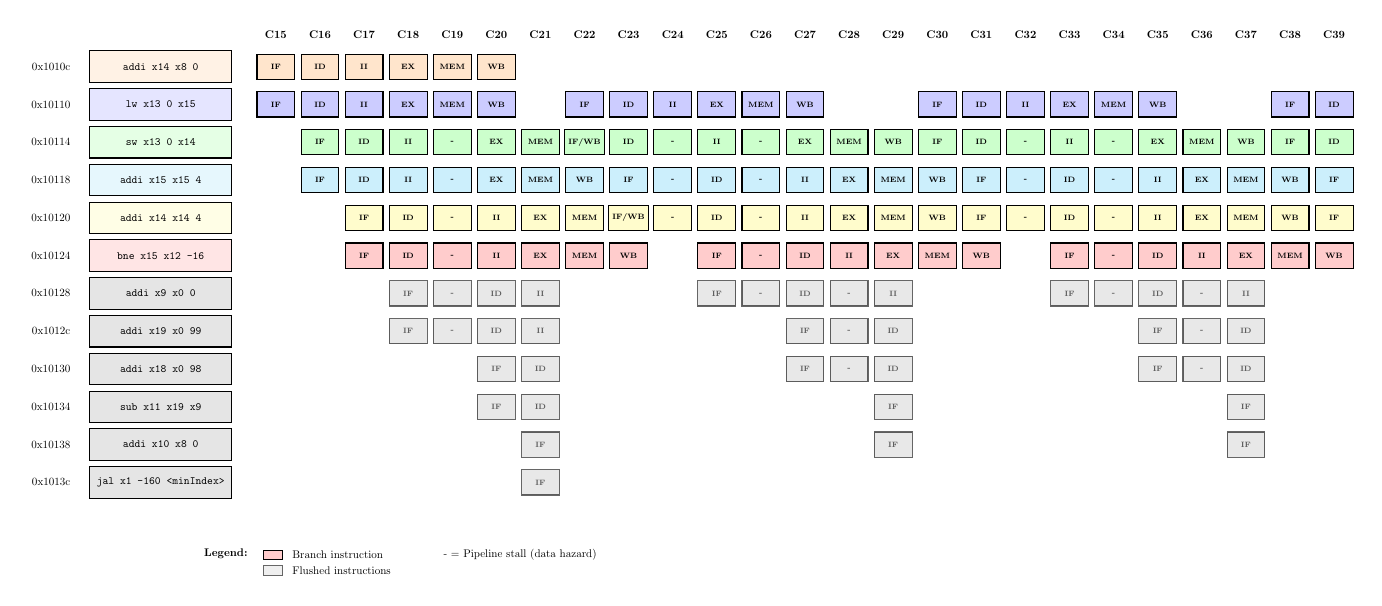
\begin{tikzpicture}[
    scale=0.4, % Ajuste l'échelle globale pour que le grand diagramme tienne sur la page
    transform shape,
    instruction/.style={rectangle, draw, minimum width=4.5cm, minimum height=1cm, font=\ttfamily\normalsize, anchor=east},
    stage/.style={draw, minimum width=1.2cm, minimum height=0.8cm, font=\scriptsize\bfseries},
    stall/.style={draw, fill=gray!20, minimum width=1.4cm, minimum height=1cm, font=\scriptsize\bfseries},
    header/.style={font=\normalsize\bfseries}
]


\foreach \i in {15,...,39} {
    \node[header] at (-1.4*14+1.4*\i, 1) {C\i};
}
% Program counter addresses
\node[anchor=east, font=\normalsize] at (-5, 0) {0x1010c};
\node[anchor=east, font=\normalsize] at (-5, -1*1.2) {0x10110};
\node[anchor=east, font=\normalsize] at (-5, -2*1.2) {0x10114};
\node[anchor=east, font=\normalsize] at (-5, -3*1.2) {0x10118};
\node[anchor=east, font=\normalsize] at (-5, -4*1.2) {0x10120};
\node[anchor=east, font=\normalsize] at (-5, -5*1.2) {0x10124};
\node[anchor=east, font=\normalsize] at (-5, -6*1.2) {0x10128};
\node[anchor=east, font=\normalsize] at (-5, -7*1.2) {0x1012c};
\node[anchor=east, font=\normalsize] at (-5, -8*1.2) {0x10130};
\node[anchor=east, font=\normalsize] at (-5, -9*1.2) {0x10134};
\node[anchor=east, font=\normalsize] at (-5, -10*1.2) {0x10138};
\node[anchor=east, font=\normalsize] at (-5, -11*1.2) {0x1013c};
% --- Libellés des Instructions ---
\node[instruction,fill=orange!10] at (0, 0) {addi x14 x8 0};
\node[instruction,fill=blue!10] at (0, -1*1.2) {lw x13 0 x15};
\node[instruction,fill=green!10] at (0, -2*1.2) {sw x13 0 x14};
\node[instruction,fill=cyan!10] at (0, -3*1.2) {addi x15 x15 4};
\node[instruction,fill=yellow!10] at (0, -4*1.2) {addi x14 x14 4};
\node[instruction,fill=red!10] at (0, -5*1.2) {bne x15 x12 -16};
\node[instruction, fill=gray!20] at (0, -6*1.2) {addi x9 x0 0};
\node[instruction, fill=gray!20] at (0, -7*1.2) {addi x19 x0 99};
\node[instruction, fill=gray!20] at (0, -8*1.2) {addi x18 x0 98};
\node[instruction, fill=gray!20] at (0, -9*1.2) {sub x11 x19 x9};
\node[instruction, fill=gray!20] at (0, -10*1.2) {addi x10 x8 0};
\node[instruction, fill=gray!20] at (0, -11*1.2) {jal x1 -160 <minIndex>};



% addi x14 x8 0
\foreach \c/\s in {1/IF, 2/ID, 3/II, 4/EX, 5/MEM, 6/WB} \node[stage, fill=orange!20] at (1.4*\c, 0) {\s};

% lw x13 0 x15
\foreach \c/\s in {1/IF, 2/ID, 3/II, 4/EX, 5/MEM, 6/WB, 8/IF, 9/ID, 10/II, 11/EX, 12/MEM, 13/WB, 16/IF, 17/ID, 18/II, 19/EX, 20/MEM, 21/WB , 24/IF ,25/ID}
    \node[stage, fill=blue!20] at (1.4*\c, -1*1.2) {\s};

% sw x13 0 x14
\foreach \c/\s in {2/IF, 3/ID, 4/II, 5/-, 6/EX, 7/MEM, 8/{IF/WB}, 9/ID, 10/-, 11/II, 12/-, 13/EX, 14/MEM, 15/WB, 16/IF, 17/ID, 18/-, 19/II, 20/-, 21/EX,22/MEM , 23/WB ,23/WB ,24/IF ,25/ID}
    \node[stage, fill=green!20] at (1.4*\c, -2*1.2) {\s};

% addi x15 x15 4
\foreach \c/\s in {2/IF, 3/ID, 4/II, 5/-, 6/EX, 7/MEM, 8/WB, 9/IF, 10/-, 11/ID, 12/-, 13/II, 14/EX, 15/MEM, 16/WB, 17/IF, 18/-, 19/ID, 20/-, 21/II, 22/EX , 23/MEM ,24/WB ,25/IF}
    \node[stage, fill=cyan!20] at (1.4*\c, -3*1.2) {\s};

% addi x14 x14 4
\foreach \c/\s in {3/IF, 4/ID, 5/-, 6/II, 7/EX, 8/MEM, 9/{IF/WB}, 10/-, 11/ID, 12/-, 13/II, 14/EX, 15/MEM, 16/WB, 17/IF, 18/-, 19/ID, 20/-, 21/II, 22/EX , 23/MEM ,24/WB ,25/IF}
    \node[stage, fill=yellow!20] at (1.4*\c, -4*1.2) {\s};

% bne x15 x12 -16
\foreach \c/\s in {3/IF, 4/ID, 5/-, 6/II, 7/EX, 8/MEM, 9/WB, 11/IF, 12/-, 13/ID, 14/II, 15/EX, 16/MEM, 17/WB, 19/IF, 20/-, 21/ID, 22/II, 23/EX, 24/MEM, 25/WB}
    \node[stage, fill=red!20] at (1.4*\c, -5*1.2) {\s};

% --- Instructions Flushed (Grisées) ---
% addi x9
\foreach \c/\s in {4/IF, 5/-, 6/ID, 7/II, 11/IF, 12/-, 13/ID, 14/-, 15/II, 19/IF, 20/-, 21/ID, 22/-, 23/II}
    \node[stage, fill=gray!30 ,opacity=0.6] at (1.4*\c, -6*1.2) {\s};

% addi x19
\foreach \c/\s in {4/IF, 5/-, 6/ID, 7/II, 13/IF, 14/-, 15/ID, 21/IF, 22/-, 23/ID}
    \node[stage, fill=gray!30 ,opacity=0.6] at (1.4*\c, -7*1.2) {\s};

% addi x18
\foreach \c/\s in {6/IF, 7/ID, 13/IF, 14/-, 15/ID, 21/IF, 22/-, 23/ID}
    \node[stage,fill=gray!30 ,opacity=0.6] at (1.4*\c, -8*1.2) {\s};

% sub x11
\foreach \c/\s in {6/IF, 7/ID, 15/IF, 23/IF}
    \node[stage, fill=gray!30 ,opacity=0.6] at (1.4*\c, -9*1.2) {\s};

% addi x10
\foreach \c/\s in {7/IF, 15/IF, 23/IF}
    \node[stage, fill=gray!30 ,opacity=0.6] at (1.4*\c, -10*1.2) {\s};

% jal x1
\node[stage, fill=gray!30 ,opacity=0.6] at (1.4*7, -11*1.2) {IF};


% Legend
\node[font=\normalsize\bfseries, anchor=north west] at (-1, -2.2-13) {\textbf{Legend:}};

\node[draw, fill=red!20, minimum width=0.6cm, minimum height=0.3cm, anchor=west] at (1.0, -2.5-13) {};
\node[font=\normalsize, anchor=west] at (1.8, -2.5-13) {Branch instruction};

\node[draw, fill=gray!20, minimum width=0.6cm, minimum height=0.3cm, opacity=0.6, anchor=west] at (1.0, -3.0-13) {};
\node[font=\normalsize, anchor=west] at (1.8, -3.0-13) {Flushed instructions};

\node[font=\normalsize, anchor=west] at (6.6, -2.5-13)  {- = Pipeline stall (data hazard)};



\end{tikzpicture}
\caption{Pipeline behavior during the array copy loop.}
\label{fig:dual_issue_hazards}
\end{figure}
A dominant factor limiting parallelism is the presence of data dependencies \cite{wall_ilp}. For instance, the instruction:

\begin{lstlisting}[style=mystyle]
lw x13, 0(x15)
\end{lstlisting}

produces a value that is immediately consumed by:

\begin{lstlisting}[style=mystyle]
sw x13, 0(x14)
\end{lstlisting}

Since the store instruction depends on the result of the load, it cannot proceed to execution before the load completes its memory stage. Even with forwarding mechanisms, load-use latency introduces unavoidable stalls. This creates visible bubbles in the pipeline and prevents effective dual issue.

Furthermore, pointer update instructions such as:

\begin{lstlisting}[style=mystyle]
addi x15, x15, 4
addi x14, x14, 4
\end{lstlisting}

are directly followed by the branch instruction:

\begin{lstlisting}[style=mystyle]
bne x15, x12, -16
\end{lstlisting}

The branch depends on the updated value of \texttt{x15}. Since branch resolution occurs only after the execute stage, the processor cannot immediately determine the next program counter value. As shown in the diagram, incorrectly fetched instructions are flushed when the branch is taken, leading to additional wasted cycles. These control hazards significantly reduce overall efficiency.

Another key observation from the diagram is that many cycles utilize only one execution slot despite the dual-issue capability. Because the processor operates in-order, an instruction that cannot be issued blocks subsequent instructions, even if they are independent. This strict ordering severely limits the exploitation of Instruction-Level Parallelism (ILP).

Overall, the pipeline behavior demonstrates that the dual-issue capability is frequently underutilized due to dependency chains and control hazards.
\subsubsection{Instruction Pairing and Issue Constraints}

Efficient instruction pairing in a dual-issue in-order processor requires the presence of independent instructions in close proximity. However, the array copy loop exhibits a strongly sequential structure. Most instructions either produce values immediately consumed by the next instruction or modify loop control variables used shortly afterward.

The issue stage performs conservative dependency checks and only allows two instructions to proceed simultaneously if no data hazards are detected and if execution resources are available. In this workload, long dependency chains effectively serialize execution.

Although the dual-issue architecture includes multiple register read and write ports to support parallel decode and write-back operations, the instruction stream rarely provides sufficient independent work to exploit these resources efficiently. Thus, the hardware capability exceeds the parallelism exposed by the program.

\subsubsection{Performance Analysis}

The measured CPI of \textbf{1.26} represents an improvement compared to the 5-stage single-issue processor, which achieved a CPI of 1.38. This corresponds to an approximate 8.7\% performance gain. While this confirms that additional parallelism is being exploited, the improvement remains far from the theoretical optimum of 0.5 CPI.

The primary limitation arises from the inherently sequential nature of the algorithm. Insertion sort contains tight dependency chains, particularly within inner loops, which restrict the availability of independent instructions. As a result, the second issue slot frequently remains unused.

Control hazards further degrade performance. The loop contains frequent branch instructions whose outcomes depend on recently computed values. Without advanced branch prediction or speculative execution mechanisms, each misprediction introduces pipeline flushing and wasted cycles.

Microarchitectural constraints also contribute to the performance gap. Since the processor executes instructions strictly in program order, it cannot dynamically reorder independent instructions to fill unused issue slots. More advanced superscalar processors employ out-of-order execution, register renaming and dynamic scheduling to overcome this limitation. In contrast, this simpler dual-issue design can only exploit ILP that naturally appears in program order.

Finally, the instruction mix plays a significant role. A considerable portion of instructions are memory operations, making the workload partially memory-bound. In such cases, increasing ALU resources does not proportionally improve performance because memory latency becomes the dominant bottleneck.


\subsubsection{Optimal CPI}

The theoretical optimal CPI of 0.5 assumes that two independent instructions are always available, that sufficient functional units exist and that no hazards or stalls occur. Achieving this level of performance requires abundant ILP, perfect branch prediction and balanced resource availability.

In practice, these conditions are not satisfied. The workload exposes limited parallelism, branch behavior introduces control penalties and structural constraints restrict simultaneous execution of certain instruction classes. Consequently, the observed CPI of 1.26 reflects a realistic balance between architectural capability and workload characteristics.

This analysis highlights an important architectural insight: increasing issue width does not automatically guarantee proportional performance improvement. The effectiveness of dual-issue execution depends strongly on the inherent parallelism of the workload and the sophistication of the microarchitectural mechanisms used to exploit it.

\subsubsection{Comparison with 5-Stage Processor}
Table~\ref{tab:processor_comparison} presents a comparison between the classical 5-stage pipeline and the 6-stage dual-issue architecture. Although the dual-issue processor offers a theoretical CPI of 0.5 compared to 1.0 for the single-issue design, this ideal 2× speedup is not achieved in practice.

The measured CPI decreases from 1.38 to 1.26, corresponding to an improvement of about 9\%. Similarly, indicating that the second issue slot is utilized in some cycles but remains frequently underused. This confirms that the workload exposes limited Instruction-Level Parallelism (ILP), preventing full exploitation of the dual-issue capability.
It is also important to note that the branch penalty increases from 2 cycles to 3 cycles due to the deeper pipeline. As a result, control hazards become slightly more expensive, partially offsetting the throughput gains provided by dual issue.


\begin{table}[H]
\centering
\renewcommand{\arraystretch}{1.4}
\rowcolors{2}{gray!10}{white}
\begin{tabular}{|p{0.2\textwidth}|p{0.2\textwidth}|p{0.2\textwidth}|p{0.2\textwidth}|}
\hline
\rowcolor{blue!20}
\textbf{Metric} & \textbf{5-Stage} & \textbf{6-Stage Dual-Issue} & \textbf{Improvement} \\
\hline
Theoretical CPI & 1.0 & 0.5 & -2.0\% \\
Achieved CPI & 1.38 & 1.26 & -1.09\% \\ 
Branch Penalty & 2 cycles & 3 cycles & +1.5\% \\
\hline
\end{tabular}
\caption{Performance comparison between processor configurations}
\label{tab:processor_comparison}
\end{table}



\section{Caches}

\subsection{Memory Analysis}

\subsubsection*{Instructions}

Each instruction in the \texttt{.text} section is fetched from memory during execution. In order to determine the total number of distinct instruction memory accesses, the address range of each function was analyzed. Since each RISC-V instruction occupies 4 bytes, the number of instructions in each function can be calculated by dividing the total byte range by 4. The results are summarized in the following table.


\begin{table}[H]
\centering
\renewcommand{\arraystretch}{1.6}
\rowcolors{2}{gray!10}{white}
\begin{tabular}{|p{3cm}|p{3.5cm}|p{3cm}|p{3cm}|}
\hline
\rowcolor{blue!20}
\textbf{Function} & \textbf{Address Range} & \textbf{Size (bytes)} & \textbf{Instructions} \\ \hline

\texttt{minIndex} & 0x10094 -- 0x100dc & 0x4c (76 bytes) & 19 \\ \hline
\texttt{main} & 0x100e0 -- 0x10180 & 0xa4 (164 bytes) & 41 \\ \hline
\texttt{\_start} & 0x10184 -- 0x101a0 & 0x20 (32 bytes) & 8 \\ \hline

\end{tabular}
\caption{Instruction memory usage per function in the \texttt{.text} section}
\end{table}

The total number of instructions in the \texttt{.text} section is 68 (words), obtained by adding the instructions from \texttt{minIndex} (19), \texttt{main} (41), and \texttt{\_start} (8). All these instructions are located within the address range \texttt{0x10094} to \texttt{0x101a0}. Therefore, this results in 68 distinct instruction memory addresses that may be read during program execution.


\subsubsection*{Data access}

\begin{itemize}
    \item \textbf{Global Variables}
\end{itemize}

The only variable stored in the \texttt{.data} section is the global array \texttt{input}. The corresponding information is presented in the following table.



\begin{table}[H]
\centering
\renewcommand{\arraystretch}{1.6}
\rowcolors{2}{gray!10}{white}
\begin{tabular}{|p{5cm}|p{6cm}|}
\hline
\rowcolor{blue!20}
\textbf{Property} & \textbf{Value} \\ \hline

Array name & \texttt{input} \\ \hline
Number of elements & 99 integers (SIZE) \\ \hline
Size of each integer & 4 bytes \\ \hline
Total size in memory & 99 $\times$ 4 = 396 bytes \\ \hline
Memory words accessed & 396 / 4 = 99 words \\ \hline

\end{tabular}
\caption{Memory characteristics of the \texttt{input} array}
\end{table}


Each element is accessed only once during the copy operation to \texttt{buf}, and the array is not referenced again afterwards. Consequently, retaining its memory blocks in the cache does not provide any performance benefit.



\begin{itemize}
    \item \textbf{Local Variables}
\end{itemize}

The \texttt{buf} array is a copy of the \texttt{input} array stored on the stack. Therefore, it has the same characteristics in terms of size, number of elements, and memory layout.

\begin{table}[H]
\centering
\renewcommand{\arraystretch}{1.6}
\rowcolors{2}{gray!10}{white}
\begin{tabular}{|p{5cm}|p{6cm}|}
\hline
\rowcolor{blue!20}
\textbf{Property} & \textbf{Value} \\ \hline

Array name & \texttt{buf} \\ \hline
Number of elements & 99 integers (SIZE) \\ \hline
Size of each integer & 4 bytes \\ \hline
Total size in memory & 99 $\times$ 4 = 396 bytes \\ \hline
Memory words accessed & 396 / 4 = 99 words \\ \hline


\end{tabular}
\caption{Memory characteristics of the \texttt{buf} array}
\end{table}

Unlike \texttt{input}, the memory locations of \texttt{buf} are accessed multiple times throughout the sorting procedure. Consequently, caching these blocks is advantageous, since it reduces memory access latency and increases the likelihood of cache hits.



\begin{itemize}
    \item \textbf{Prologue and Epilogue}
\end{itemize}

In the \texttt{main} function, several memory accesses to the stack occur as part of the function prologue and epilogue. At the beginning of the function, five \texttt{sw} instructions store the registers \texttt{ra}, \texttt{s0}, \texttt{s1}, \texttt{s2}, and \texttt{s3} onto the stack in order to preserve their values. At the end of the function, six \texttt{lw} instructions restore these registers (as well as the return value register \textbf{a0}) from the stack. Altogether, this results in 11 additional data memory accesses, which would be made on 6 different memory positions  caused by stack operations within \texttt{main}.


\begin{lstlisting}
sw ra,428(sp)  lw a0,4(sp)     lw s3,412(sp)
sw s0,424(sp)  lw ra,428(sp)
sw s1,420(sp)  lw s0,424(sp)
sw s2,416(sp)  lw s1,420(sp)
sw s3,412(sp)  lw s2,416(sp)
\end{lstlisting}

Similarly, the \texttt{\_start} function also performs stack access. In this case, a single \texttt{sw} instruction stores the return address register (\texttt{ra}) onto the stack. This contributes one additional data memory access. Therefore, the stack operations in \texttt{\_start} account for one extra memory access during execution.

\begin{lstlisting}
sw ra,12(sp)
\end{lstlisting}

This leads to a total of 7 additional distinct memory addresses that may be accessed during execution.



\begin{itemize}
    \item \textbf{Data access conclusion}
\end{itemize}

Considering the 99 memory locations corresponding to the global \texttt{input} array, the 99 locations of the local \texttt{buf} array, and the 7 stack locations involved in load and store operations, the program may access up to 205 distinct data memory addresses during execution.
This corresponds to the particular case under study. More generally, the total number of distinct data memory locations accessed during execution can be described by the expression $2N + 7$, where $N$ denotes the number of elements in each array and 7 represents the stack-related memory accesses.


\subsection{Speculations about the cache}



\subsubsection*{Data Cache}

In this case, it is known that up to 205 distinct data memory locations may be accessed during execution. Therefore, in order to minimize capacity misses and reduce potential conflicts due to insufficient cache space, it is reasonable to configure the cache with at least 205 available slots. Since cache sizes are typically powers of two, the closest higher power of two is 256 (2\textsuperscript{8}). 

Accordingly, a configuration with 2\textsuperscript{4} lines (16 sets), 2\textsuperscript{2} ways (4-way associativity), and 2\textsuperscript{2} blocks per line (4 words per block) is proposed. This results in a total cache size of 9984 bits. Under this configuration, the execution produces 10\,448 hits and 53 misses.

\begin{table}[H]
\centering
\renewcommand{\arraystretch}{1.6}
\rowcolors{2}{gray!10}{white}
\begin{tabular}{|p{5cm}|p{6cm}|}
\hline
\rowcolor{blue!20}
\textbf{Parameter} & \textbf{Value} \\ \hline

$2^N$ Lines & $2^4 = 16$ \\ \hline
$2^N$ Ways & $2^2 = 4$ \\ \hline
$2^N$ Blocks & $2^2 = 4$ \\ \hline
Total size & 9920 bits \\ \hline
Hit rate & 0.995 \\ \hline
Hits & 10\,448 \\ \hline
Misses & 53 \\ \hline
Writebacks & 301 \\ \hline
\end{tabular}
\caption{Proposed data cache configuration and simulation results}
\end{table}



\subsubsection*{Instruction Cache}

For the instruction cache, a total of 68 distinct instruction memory locations are accessed. To avoid capacity-related misses and ensure sufficient cache space, the next power of two greater than 68 is selected, namely 128 (2\textsuperscript{7}). 

To achieve this, a configuration with 16 lines (2\textsuperscript{4}), 2 ways (2\textsuperscript{1}), and 4 blocks per line (2\textsuperscript{2}) is proposed. This results in a total cache size of 4928 bits. With this configuration, the following performance metrics were obtained.


\begin{table}[H]
\centering
\renewcommand{\arraystretch}{1.6}
\rowcolors{2}{gray!10}{white}
\begin{tabular}{|p{5cm}|p{6cm}|}
\hline
\rowcolor{blue!20}
\textbf{Instruction Cache Parameter} & \textbf{Value} \\ \hline

$2^N$ Lines & $2^4 = 16$ \\ \hline
$2^N$ Ways & $2^1 = 2$ \\ \hline
$2^N$ Blocks & $2^2 = 4$ \\ \hline
Total size & 4928 bits \\ \hline
Hit rate & 0.9996 \\ \hline
Hits & 42754 \\ \hline
Misses & 17 \\ \hline
Writebacks & 0 \\ \hline
\end{tabular}
\caption{Proposed Instruction cache configuration and simulation results}
\end{table}



\subsection{Cache analysis}





\subsubsection*{Instruction Cache}

\paragraph{Instruction Cache Capacity Selection}\mbox{}\\

First, the number of cache slots must be determined in order to reduce capacity misses and ensure that each instruction can be mapped without unnecessary conflicts. In this case, there are 68 instructions. To avoid capacity limitations, the cache should be able to contain at least this number of instruction words. Since cache parameters are typically powers of two, the next power of two greater than 68 is 128, which corresponds to $2^{7}$.

The total number of cache blocks is determined by:

\[
2^{L} \times 2^{W} \times 2^{B}
\]

where:
\begin{itemize}
    \item $L$ is the number of index bits (number of sets),
    \item $W$ is the associativity (number of ways),
    \item $B$ corresponds to the block offset bits (block size).
\end{itemize}

Therefore, to obtain a total capacity of 128 instruction words, the following condition must hold:

\[
2^{L} \cdot 2^{W} \cdot 2^{B} = 2^{7}
\quad \Longleftrightarrow \quad
L + W + B = 7
\]


This guarantees that the cache has sufficient capacity (128 instruction words) to store all 68 instructions while minimizing capacity misses.


\paragraph{Block Organization and Compulsory Miss Reduction}\mbox{}\\

Once the total cache capacity has been defined, capacity misses are no longer a concern. The next step is to determine the block organization in order to reduce compulsory misses when accessing new instruction addresses.

Since all instructions are stored consecutively in memory, spatial locality can be fully exploited. Therefore, the most straightforward solution is to define a block size large enough so that all instructions are fetched when the first instruction is loaded into the cache. In this way, only one compulsory miss occurs during the initial access, and all subsequent instruction accesses result in cache hits.

Based on this reasoning, the following configuration is proposed:

\begin{itemize}
    \item 1 line (set)
    \item 1 way (direct-mapped)
    \item 128 words per block
\end{itemize}

This configuration allows the entire instruction sequence to be stored in a single cache block, ensuring that after the first miss, all instructions remain accessible without additional compulsory misses.

The resulting total cache size for this configuration is 4121 bits.

\begin{table}[H]
\centering
\renewcommand{\arraystretch}{1.4}
\rowcolors{2}{gray!10}{white}
\begin{tabular}{|p{4cm}|p{4cm}|}
\hline
\rowcolor{blue!20}
\textbf{Parameter} & \textbf{Value} \\
\hline
Lines & $2^{0} = 1$ \\
Ways & $2^{0} = 1$ \\
Blocks (Block Size) & $2^{7} = 128$ \\
Total Size (bits) & 4121 \\
Cache Hits & 42770 \\
Cache Misses & 1 \\
\hline
\end{tabular}
\caption{Instruction Cache Configuration and Performance Results}
\label{tab:icache_config}
\end{table}



\subsubsection*{Data Cache}



\paragraph{Data Cache Capacity Selection}\mbox{}\\


In this case, a similar approach is applied. Since 205 memory positions are accessed, the cache must have sufficient capacity to avoid capacity misses caused by insufficient space.

Therefore, the minimum required capacity must be at least 205 data words. As cache configurations are defined in powers of two, the next power of two greater than 205 is 256, which corresponds to $2^{8}$.

Thus, the cache parameters must satisfy:

\[
2^{L} \cdot 2^{W} \cdot 2^{B} = 2^{8}
\quad \Longleftrightarrow \quad
L + W + B = 8
\]

This guarantees that the cache has enough total capacity (256 data words) to accommodate all accessed memory positions while minimizing capacity misses.


\paragraph{Data Cache Organization and Compulsory Miss Reduction - First approach (Reducing memory)}\mbox{}\\

In this case, three different memory regions are accessed during execution: the input array, the buffer array (buf), and the stack (used during the function prologue and epilogue).

Since each of these memory regions is stored contiguously in memory, spatial locality can be exploited by selecting a block size large enough to contain each array within a single block. Based on this reasoning, a configuration with $2^{7}$ blocks (128 words per block) and 2 ways is proposed. The use of two ways allows different memory regions to coexist within the same set without immediate replacement.

However, with this configuration, the total cache capacity is not sufficient to simultaneously store the entire input array, the buffer array, and the stack accesses. As a result, at least three compulsory misses will occur:

\begin{itemize}
    \item One compulsory miss when the input array is first accessed.
    \item One compulsory miss when the buffer array is first accessed.
    \item One compulsory miss when the stack region (prologue/epilogue accesses) is first accessed.
\end{itemize}

After these initial compulsory misses, additional misses may occur due to capacity limitations if the three memory regions compete for cache space and cannot coexist simultaneously.


\begin{table}[H]
\centering
\renewcommand{\arraystretch}{1.4}
\rowcolors{2}{gray!10}{white}
\begin{tabular}{|p{4cm}|p{4cm}|}
\hline
\rowcolor{blue!20}
\textbf{Parameter} & \textbf{Value} \\
\hline
Lines & $2^{0} = 1$ \\
Ways & $2^{1} = 2$ \\
Blocks (Block Size) & $2^{7} = 128$ \\
Total Size (bits) & 8244 \\
Cache Hits & 10498 \\
Cache Misses & 3 \\
\hline
\end{tabular}
\caption{Data Cache Configuration and Performance Results}
\label{tab:dcache_config}
\end{table}


\paragraph{Data Cache Organization and Compulsory Miss Reduction - Second approach (Reducing misses)}\mbox{}\\

While analyzing the results, we noticed that an alternative strategy could be applied: reducing misses by increasing the block size, even at the cost of a larger cache.

The main idea is to use a larger block so that all stack-related accesses (including the \texttt{buf} region as well as the function prologue and epilogue accesses) are captured within the same cache block. With this approach, increasing the block size to 256 words ($2^{8}$) reduces the number of misses to 2:
\begin{itemize}
    \item One miss when the input region is accessed for the first time.
    \item One miss when the stack region is first accessed (prologue/epilogue and related stack accesses).
\end{itemize}

This configuration improves performance by reducing the number of first-time block fetches, but it increases the cache size due to the larger block.

\medskip

The resulting configuration and performance metrics are summarized in Table~\ref{tab:dcache_alt_256}.

\begin{table}[H]
\centering
\renewcommand{\arraystretch}{1.4}
\rowcolors{2}{gray!10}{white}
\begin{tabular}{|p{4cm}|p{4cm}|}
\hline
\rowcolor{blue!20}
\textbf{Parameter} & \textbf{Value} \\
\hline
Lines & $2^{0} = 1$ \\
Ways & $2^{1} = 2$ \\
Blocks (Block Size) & $2^{8} = 256$ \\
Total Size (bits) & 16434 \\
Cache Hits & 10499 \\
Cache Misses & 2 \\
\hline
\end{tabular}
\caption{Alternative Data Cache Configuration (256-word Block) and Performance Results}
\label{tab:dcache_alt_256}
\end{table}

\subsection{Proposed Efficiency Metric}



In order to evaluate the efficiency of each cache configuration, a metric that combines performance and hardware cost is required. Let $M$ denote the total number of misses, $A$ the total number of memory accesses, and $S$ the cache size in bits. The miss rate is defined as:

\[
r_M = \frac{M}{A}
\]

This quantity represents the probability that a memory access results in a cache miss. To incorporate the hardware cost into the evaluation, we define the following efficiency metric:

\[
E = r_M \cdot S = \frac{M}{A} \cdot S
\]

This metric penalizes both high miss rates and large hardware sizes. A configuration with a low miss rate but excessively large size may not be efficient, just as a small cache with a high miss rate may lead to poor performance. Therefore, minimizing $E$ provides a balanced trade-off between cache performance and implementation cost, allowing for a fair comparison between different configurations without introducing additional weighting parameters.

\paragraph{Instruction Cache Configuration Comparison}\mbox{}\\

Two instruction cache configurations were evaluated in order to determine the most efficient design according to the proposed metric.

\medskip

\begin{table}[H]
\centering
\renewcommand{\arraystretch}{1.4}
\rowcolors{2}{gray!10}{white}
\begin{tabular}{|p{5cm}|p{3cm}|p{3cm}|}
\hline
\rowcolor{blue!20}
\textbf{Parameter} & \textbf{Configuration 1} & \textbf{Configuration 2} \\
\hline
Lines & $2^{0} = 1$ & $2^{1} = 2$ \\
Ways & $2^{0} = 1$ & $2^{1} = 2$ \\
Blocks (Block Size) & $2^{7} = 128$ & $2^{4} = 16$ \\
Size (bits) & 4121 & 2160 \\
Total Accesses ($A$) & 42771 & 42771 \\
Misses ($M$) & 1 & 6 \\
Miss Rate ($r = M/A$) & $2.34 \times 10^{-5}$ & $1.40 \times 10^{-4}$ \\
Efficiency Metric ($E = r \cdot S$) & 0.0963 & 0.303 \\
\hline
\end{tabular}
\caption{Instruction Cache Configuration and Efficiency Comparison}
\label{tab:icache_comparison_full}
\end{table}

\medskip

Since $E_1 < E_2$, Configuration 1 is more efficient according to the defined metric. Although it requires a larger hardware size, the significant reduction in miss rate compensates for the increase in cache size.

Given the high number of instruction accesses, even a small increase in the number of misses has a measurable impact on overall efficiency. Therefore, for the instruction cache, minimizing misses proves to be more beneficial than reducing hardware size.


\paragraph{Data Cache Configuration Comparison}\mbox{}\\

Two data cache configurations were evaluated using the proposed efficiency metric.

\medskip

\begin{table}[H]
\centering
\renewcommand{\arraystretch}{1.4}
\rowcolors{2}{gray!10}{white}
\begin{tabular}{|p{5cm}|p{3cm}|p{3cm}|}
\hline
\rowcolor{blue!20}
\textbf{Parameter} & \textbf{Configuration 1} & \textbf{Configuration 2} \\
\hline
Lines & $2^{0} = 1$ & $2^{0} = 1$ \\
Ways & $2^{1} = 2$ & $2^{1} = 2$ \\
Blocks (Block Size) & $2^{7} = 128$ & $2^{8} = 256$ \\
Size (bits) & 8244 & 16343 \\
Total Accesses ($A$) & 10501 & 10501 \\
Misses ($M$) & 3 & 2 \\
Miss Rate ($r = M/A$) & $2.86 \times 10^{-4}$ & $1.90 \times 10^{-4}$ \\
Efficiency Metric ($E = r \cdot S$) & 2.35 & 3.11 \\
\hline
\end{tabular}
\caption{Data Cache Configuration and Efficiency Comparison}
\label{tab:dcache_comparison_full}
\end{table}


\medskip

Since $E_1 < E_2$, Configuration 1 provides a better balance between performance and hardware cost. Although Configuration 2 slightly reduces the number of misses, the significant increase in cache size does not justify the marginal improvement in miss rate.


\subsection{Cache miss}
In this subsection we are focusing in on illustrating different scenarios of cache misses (compulsory,
capacity and conflict) using the \textbf{Ripes} simulator. Compulsory misses are the type of cache miss
which occurs when a block of data is accessed for the first time and has never been loaded into the cache.
This kind of miss is unavoidable and occurs in any configuration of cache.

For example for a data cache configuration of 1KB total size with 2 lines, 4 way associative and block
sizes of 16 bytes exhibits a compulsory miss when the \textbf{sw x1 12 x2} instruction is executed from
the \_start function, as depicted in \ref{fig:compulsory_miss}. Another example of compulsory miss would
happen when the program reaches main and the processor executes \textbf{sw x1 428 x2}.

\begin{figure}[h]
    \centering
    \includegraphics[width=0.9\linewidth]{img/compulsory-cache-miss.png}
    \caption{Compulsory miss on data cache when executing \_start function}
    \label{fig:compulsory_miss}
\end{figure}

When speaking of conflict misses, they occur when multiple blocks of data compete for the same cache line due to
the cache's mapping scheme. For instance, in a direct-mapped cache, if two different memory addresses map to the same
cache line, they will evict each other, leading to conflict misses.

In an instruction cache configuration of 47B with 2 lines, 2 way associative and 2 blocks the following
instructions will cause conflict misses, as per figure \ref{fig:conflict_miss}:

\begin{lstlisting}
	10184:	addi x2 x2 -16
        100f0:	sw x18 416 x2
\end{lstlisting}

\begin{figure}[h]
    \centering
    \includegraphics[width=0.9\linewidth]{img/conflict-cache-miss.png}
    \caption{Conflict miss on instruction cache when executing \_start and main functions}
    \label{fig:conflict_miss}
\end{figure}

\newpage
Finally, capacity misses occur when the cache cannot contain all the blocks needed during execution, even if there are no conflicts.
This happens when the working set of the program exceeds the total cache size. For example, if we have a data
cache of 1KB total size with 2 lines, 4 way associative and block sizes of 16 bytes, and the program accesses
more than 64 bytes of data (which is the total capacity of the cache), it will result in capacity misses.

This is illustrated in figure \ref{fig:capacity_miss} when the program executes the following instructions:
\begin{figure}[h]
    \centering
    \includegraphics[width=0.9\linewidth]{img/capacity-cache-miss.png}
    \caption{Capacity miss on data cache when executing main functions}
    \label{fig:capacity_miss}
\end{figure}

\newpage
\subsection{Write Allocate vs No Write Allocate}

When using write allocate (WA), the cache line is loaded into the cache on a write miss before the
store operation is performed. A concrete example of this behavior can be observed when copying data
from the input array to the buf array in the first loop of the main function. Consider the first store
to a new line of the destination. Destination addresses written: $D+0$, $D+4$, $D+8$, $D+12$, $D+16$, ...

For the first store to $D+0$:
\begin{itemize}
    \item \texttt{sw D+0} $\rightarrow$ write miss
    \item With WA: cache fetches whole line into L1
    \item Then performs store into the line $\rightarrow$ line is now dirty
    \item The next stores ($D+4$, $D+8$ ...) are write hits (fast, no extra line fetches)
\end{itemize}

So per 16B line, you pay one line fill, then get cheap hits.

When using no write allocate (NWA), the cache does not load the line on a write miss. Instead, it
writes the data directly to memory. Therefore, this will yield to a different cost per write in the
case of the above mentioned for loop.

First store to $D+0$:
\begin{itemize}
    \item \texttt{sw D+0} $\rightarrow$ write miss
    \item With NWA: do not load the line
    \item The word is written to memory
\end{itemize}

Next store to $D+4$:
\begin{itemize}
    \item still a miss, still write-around
\end{itemize}

\begin{figure}[h]
    \centering
    \includegraphics[width=0.9\linewidth]{img/write-allocate.png}
    \caption{WA: stack addresses appear, block 1 hit, by write-allocate}
    \label{fig:write-allocate}
\end{figure}

\begin{figure}[h]
    \centering
    \includegraphics[width=0.9\linewidth]{img/write-allocate-2.png}
    \caption{WA: stack addresses appear, block 0 miss, compulsory}
    \label{fig:write-allocate-2}
\end{figure}

In the next figure the NWA policy is illustrated. As it can be seen no stack addresses appear, even if
the same instructions are executed. This is because the cache is not loading the line on a write miss,
but instead writing directly to memory.

\begin{figure}[h]
    \centering
    \includegraphics[width=0.9\linewidth]{img/no-write-allocate.png}
    \caption{NWA: no stack addresses appear, all writes are cache miss}
    \label{fig:no-write-allocate}
\end{figure}





%%%%%%%%%%%%%%%%%%%%%%%%%%%%%%%%%%%%%%%%%%%%%%%%%%%%%%%%%%%%%%%%%
% SECTION BIBLIOGRAPHY
%%%%%%%%%%%%%%%%%%%%%%%%%%%%%%%%%%%%%%%%%%%%%%%%%%%%%%%%%%%%%%%%
\clearpage

\newpage % keep bibliography on a new page

\bibliographystyle{plain}   % choose a style
\bibliography{ref}      % name of .bib file (no .bib extension)

\end{document}
